\documentclass[11pt]{article}

\usepackage[T1]{fontenc}
\usepackage[utf8]{inputenc}
\usepackage{amsmath,amssymb,amsthm,mathtools,bm}
\usepackage{newtxtext,newtxmath}
\usepackage{microtype}
\usepackage[letterpaper,margin=1.02in,headheight=15pt]{geometry}
\usepackage{array,booktabs,longtable,tabularx}
\usepackage{enumitem}
\usepackage{xcolor}
\usepackage{graphicx}
\usepackage{tikz}
\usetikzlibrary{arrows.meta,calc,positioning,decorations.pathreplacing}
\usepackage{algorithm}
\usepackage[noend]{algpseudocode}
\usepackage[most]{tcolorbox}
\usepackage{fancyhdr}
\usepackage{lastpage}
\usepackage{hyperref}
\makeatletter
\providecommand*{\theHALG@line}{}
\renewcommand*{\theHALG@line}{\thealgorithm.\arabic{ALG@line}}
\makeatother
\usepackage[nameinlink,capitalise,noabbrev]{cleveref}
% Canonical mathematical notation for active FabiusFunction LaTeX documents.
%
% This file is intentionally a plain TeX input rather than a LaTeX package.
% Every standalone document loads it by an explicit path relative to that
% document's directory; included fragments inherit the definitions from their
% root document.  Keep this file independent of document layout and metadata.
%
% Contract:
%   * one command has one mathematical meaning throughout the active corpus;
%   * names encode semantic roles rather than a document-local choice of letter;
%   * visually similar but differently normalized objects have different print;
%   * every command below is defined normatively in the notation catalogue.
%
% The active corpus excludes docs/archive/.  Historical sources may retain
% their original notation only inside an explicitly labelled quotation.

\makeatletter
\@ifundefined{mathbb}{%
  \PackageError{fabius-notation}{The amssymb package must be loaded first}%
    {Load amsmath and amssymb before inputting fabius-notation.tex.}%
}{}
\@ifundefined{operatorname}{%
  \PackageError{fabius-notation}{The amsmath package must be loaded first}%
    {Load amsmath before inputting fabius-notation.tex.}%
}{}
\makeatother

% Version stamp used by the catalogue and by static audits.
\newcommand{\FabiusNotationVersion}{2026-08-31}

% Number systems.  NaturalNumbers is explicitly the nonnegative convention.
\newcommand{\NaturalNumbers}{\mathbb{N}_{0}}
\newcommand{\PositiveIntegers}{\mathbb{N}_{>0}}
\newcommand{\IntegerNumbers}{\mathbb{Z}}
\newcommand{\RationalNumbers}{\mathbb{Q}}
\newcommand{\RealNumbers}{\mathbb{R}}
\newcommand{\ComplexNumbers}{\mathbb{C}}
\newcommand{\ExtendedRealNumbers}{\overline{\mathbb{R}}}

% The three principal Fabius--Rvachev functions.  Subscripts are deliberate:
% a bare F and a calligraphic F have several unrelated uses in the corpus.
\newcommand{\FabiusBounded}{F_{\mathrm{bd}}}
\newcommand{\FabiusGlobal}{F_{\mathrm{gl}}}
\newcommand{\FabiusQuantile}{Q_{F}}
\newcommand{\FabiusClampedQuantile}{Q_{F,\mathrm{cl}}}
\newcommand{\RvachevUp}{\operatorname{up}}

% Constants, elementary operators, and delimiters.
\newcommand{\EulerE}{\mathrm{e}}
\newcommand{\ImaginaryUnit}{\mathrm{i}}
\newcommand{\Differential}{\mathop{}\!\mathrm{d}}
\newcommand{\AbsoluteValue}[1]{\left\lvert #1\right\rvert}
\newcommand{\Norm}[1]{\left\lVert #1\right\rVert}
\newcommand{\Floor}[1]{\left\lfloor #1\right\rfloor}
\newcommand{\Ceiling}[1]{\left\lceil #1\right\rceil}
\newcommand{\FractionalPart}[1]{\left\{#1\right\}}
\newcommand{\PositivePart}[1]{\left(#1\right)_{+}}
\newcommand{\IndicatorOf}[1]{\mathbf{1}_{#1}}
\newcommand{\SetOf}[1]{\left\{#1\right\}}
\newcommand{\InnerProduct}[1]{\left\langle #1\right\rangle}
\newcommand{\CardinalityOf}[1]{\left\lvert #1\right\rvert}
\newcommand{\DefinitionEquals}{\mathrel{\coloneqq}}
\newcommand{\Sign}{\operatorname{sgn}}
\newcommand{\IdentityOperator}{\operatorname{id}}
\newcommand{\SpanOperator}{\operatorname{span}}
\newcommand{\TraceOperator}{\operatorname{tr}}
\newcommand{\RankOperator}{\operatorname{rank}}
\newcommand{\DiagonalOperator}{\operatorname{diag}}
\newcommand{\ResidueOperator}{\operatorname*{Res}}
\newcommand{\LeastCommonMultiple}{\operatorname{lcm}}
\newcommand{\OrderOperator}{\operatorname{ord}}
\newcommand{\PrincipalLogarithm}{\operatorname{Log}}
\newcommand{\FallingFactorial}[2]{\left(#1\right)^{\underline{#2}}}
\newcommand{\RisingFactorial}[2]{\left(#1\right)^{\overline{#2}}}

% Support, topology, convolution, and metric notation.
\newcommand{\SupportOperator}{\operatorname{supp}}
\newcommand{\SupportOf}[1]{\SupportOperator\!\left(#1\right)}
\newcommand{\TopologicalSupportOf}[1]{\operatorname{tsupp}\!\left(#1\right)}
\newcommand{\Convolution}{\mathbin{*}}
\newcommand{\MetricDistance}{\operatorname{dist}}
\newcommand{\TotalVariationDistance}{d_{\mathrm{TV}}}

% Probability.  Equality and convergence in law are not metric distance.
\newcommand{\Probability}{\mathbb{P}}
\newcommand{\Expectation}{\mathbb{E}}
\newcommand{\Variance}{\operatorname{Var}}
\newcommand{\Covariance}{\operatorname{Cov}}
\newcommand{\LawOperator}{\operatorname{Law}}
\newcommand{\LawOf}[1]{\LawOperator\!\left(#1\right)}
\newcommand{\EqualInLaw}{\mathrel{\overset{\mathrm{law}}{=}}}
\newcommand{\ConvergesInLaw}{\mathrel{\xrightarrow{\mathrm{law}}}}

% Fourier and integral transforms.  The printed labels expose normalization.
% FourierTwoPi uses exp(-2*pi*i*x*xi); FourierAngular uses exp(-i*x*omega).
\newcommand{\FourierTwoPi}[1]{\widehat{#1}_{\,2\pi}}
\newcommand{\FourierAngular}[1]{\widehat{#1}_{\,\mathrm{ang}}}
\newcommand{\LaplaceTransformSymbol}{\mathcal{L}}
\newcommand{\MellinTransformSymbol}{\mathcal{M}}
\newcommand{\LaplaceTransformOf}[1]{\LaplaceTransformSymbol\!\left[#1\right]}
\newcommand{\MellinTransformOf}[1]{\MellinTransformSymbol\!\left[#1\right]}
\newcommand{\MomentGeneratingFunction}[1]{M_{#1}}
\newcommand{\CharacteristicFunction}[1]{\varphi_{#1}}

% The two standard sinc functions must never share one symbol.
\newcommand{\SincRad}{\operatorname{sinc}_{\mathrm{rad}}}
\newcommand{\SincPi}{\operatorname{sinc}_{\pi}}

% Binary arithmetic and Thue--Morse notation.
\newcommand{\BinaryDigitSum}{\operatorname{wt}_{2}}
\newcommand{\ThueMorseSignSymbol}{\varepsilon}
\newcommand{\ThueMorseSign}[1]{\varepsilon_{#1}}
\newcommand{\PadicValuation}[1]{\nu_{#1}}
\newcommand{\TwoAdicValuation}{\nu_{2}}

% q-series notation.  Every base is an explicit argument.
\newcommand{\QPochhammer}[3]{\left(#1;#2\right)_{#3}}
\newcommand{\GaussianBinomial}[3]{%
  \genfrac{[}{]}{0pt}{}{#1}{#2}_{#3}%
}
\newcommand{\QInteger}[2]{\left[#1\right]_{#2}}

% Named special functions.
\newcommand{\Polylogarithm}{\operatorname{Li}}
\newcommand{\LambertW}{W}
\newcommand{\GammaFunction}{\Gamma}
\newcommand{\RiemannZeta}{\zeta}

% Asymptotics.  BigO and LittleO are operator tokens for existing formula
% grammar; prefer the At forms so that the limiting regime is printed.
\newcommand{\BigO}{\mathcal{O}}
\newcommand{\LittleO}{o}
\newcommand{\BigOAt}[2]{\mathcal{O}_{#2}\!\left(#1\right)}
\newcommand{\LittleOAt}[2]{o_{#2}\!\left(#1\right)}


\definecolor{Ink}{HTML}{17202A}
\definecolor{DeepBlue}{HTML}{244A64}
\definecolor{SoftBlue}{HTML}{EAF2F7}
\definecolor{DeepGreen}{HTML}{2F5D50}
\definecolor{SoftGreen}{HTML}{EDF5F0}
\definecolor{WarmGray}{HTML}{F4F1EA}
\definecolor{RuleGray}{HTML}{B9C2C9}
\definecolor{Brick}{HTML}{8B3E2F}

\hypersetup{
  colorlinks=true,
  linkcolor=DeepBlue,
  citecolor=DeepGreen,
  urlcolor=Brick,
  pdfauthor={},
  pdftitle={Polynomial-Logarithmic Transseries: Algebra, Composition, Reversion, and Lambert W},
  pdfsubject={Formal and asymptotic calculus of inverse-power series with polynomial logarithmic coefficients}
}

\pagestyle{fancy}
\fancyhf{}
\fancyhead[L]{\small Polynomial-logarithmic transseries}
\fancyhead[R]{\small\nouppercase{\leftmark}}
\fancyfoot[C]{\small \thepage\ of \pageref{LastPage}}
\renewcommand{\headrulewidth}{0.35pt}

\setcounter{secnumdepth}{3}
\setcounter{tocdepth}{2}
\setlength{\parindent}{1.15em}
\setlength{\parskip}{0.22em}
\setlist{itemsep=0.25em,topsep=0.45em}
\allowdisplaybreaks[2]

\newtheoremstyle{pltheorem}
  {0.8em}{0.8em}{\itshape}{}{}{.}{0.6em}{}
\theoremstyle{pltheorem}
\newtheorem{theorem}{Theorem}[section]
\newtheorem{proposition}[theorem]{Proposition}
\newtheorem{lemma}[theorem]{Lemma}
\newtheorem{corollary}[theorem]{Corollary}
\newtheorem{definition}[theorem]{Definition}
\newtheorem{example}[theorem]{Example}
\newtheorem{remark}[theorem]{Remark}

\newtcolorbox{keybox}[1][]{
  enhanced,breakable,colback=SoftBlue,colframe=DeepBlue,
  boxrule=0.65pt,arc=1.4mm,left=1.5mm,right=1.5mm,top=1.1mm,bottom=1.1mm,
  title={#1},fonttitle=\bfseries
}
\newtcolorbox{warningbox}[1][]{
  enhanced,breakable,colback=WarmGray,colframe=Brick,
  boxrule=0.65pt,arc=1.4mm,left=1.5mm,right=1.5mm,top=1.1mm,bottom=1.1mm,
  title={#1},fonttitle=\bfseries
}
\newtcolorbox{algorithmbox}[1][]{
  enhanced,breakable,colback=SoftGreen,colframe=DeepGreen,
  boxrule=0.65pt,arc=1.4mm,left=1.5mm,right=1.5mm,top=1.1mm,bottom=1.1mm,
  title={#1},fonttitle=\bfseries
}

\newcommand{\K}{\mathbb K}
\newcommand{\PL}{\PolynomialLogPowerSeriesRing{\K}}
\newcommand{\PLL}{\PolynomialLogLaurentRing{\K}}
\newcommand{\QPL}{\RationalLogLaurentField{\K}}
\newcommand{\Gnear}{\NearIdentityPolynomialLogGroup{\K}}
\newcommand{\ordt}{\nu_t}
\newcommand{\lm}{\operatorname{lm}}
\newcommand{\lc}{\operatorname{lc}}
\newcommand{\rev}{\langle-1\rangle_{\circ}}
\newcommand{\stirlingone}[2]{\genfrac{[}{]}{0pt}{}{#1}{#2}}
\newcommand{\D}{\mathcal D}
\newcommand{\compose}{\mathbin{\circ}}
\newcommand{\LambertWTruncation}[1]{\LambertW^{\mathrm{tr}}_{#1}}
\newcommand{\LagrangeAuxiliaryParameter}{\varepsilon_{\mathrm{Lag}}}
\newcommand{\LogarithmOnBranch}[2]{%
  \PrincipalLogarithm_{#1}\!\left(#2\right)%
}

\crefname{equation}{equation}{equations}
\Crefname{equation}{Equation}{Equations}

\title{\textbf{Polynomial-Logarithmic Transseries}\\[0.3em]
\Large Algebra, Composition, Series Reversal, and the Lambert \(\LambertW\) Function}
\author{}
\date{August 31, 2026}

\begin{document}
\maketitle
\vspace{-2.0em}

\begin{abstract}
Polynomial-logarithmic transseries are formal expansions in inverse powers of a large variable whose coefficients are polynomials in its logarithm.  After the change of variable
\(x=\log z\), the classical large-argument expansion of the Lambert \(\LambertW\) function is the canonical example:
\[
 \LambertW(z)=x-\log x+\frac{\LambertPolynomial{1}(\log x)}{x}
      +\frac{\LambertPolynomial{2}(\log x)}{x^2}+\cdots .
\]
This article develops the corresponding algebra from first principles.  We distinguish the polynomial-logarithmic ring from the field extensions needed for unrestricted division; formulate its valuation, support geometry, differential calculus, and truncation topology; derive exact coefficient algorithms for multiplication, reciprocal, quotient, powers, logarithms, and exponentials; and give two equivalent calculi for composition with a near-identity inner series.  Series reversal is treated by a triangular coefficient recursion, a Newton method with precision doubling, and a Lagrange--B\"urmann formula adapted to expansions at infinity.

The inverse of \(x+\log x\) leads to a distinguished family of Lambert polynomials.  We derive their implicit generating equation, differential recurrence, operator formula, explicit expression through unsigned Stirling cycle numbers, Laplace transform, and numerical behavior.  The same polynomials govern every branch of the large-argument Lambert \(\LambertW\) expansion, the real branch \(\LambertW_{-1}\) near the origin, and the generalized inverse of \(y^\alpha\EulerE^y\).  Throughout, formal identities are separated from analytic asymptotics and actual convergence, and the exact points at which one must enlarge the one-logarithm class are made explicit.
\end{abstract}

\begin{keybox}[Guiding convention]
Unless stated otherwise, \(x\to+\infty\),
\[
 t=x^{-1},\qquad L=\log x,
\]
and \(\K\) is a field of characteristic zero.  A coefficient such as \(p_n(L)\) is an honest polynomial in the formal symbol \(L\).  The relation \(L=\log x\) enters through differentiation and composition, not by treating \(t\) and \(L\) as algebraically independent analytic variables.
\end{keybox}

\tableofcontents
\newpage

\section{Why this particular transseries class matters}
\label{sec:motivation}

\subsection{\texorpdfstring{From Lambert \(\LambertW\) to a one-logarithm algebra}{From Lambert W to a one-logarithm algebra}}

The Lambert function is defined branchwise by
\begin{equation}\label{eq:W-definition}
 \LambertW_k(z)\EulerE^{\LambertW_k(z)}=z.
\end{equation}
Fix compatible analytic logarithm branches \(\mathcal B_W\) and
\(\mathcal B_\xi\) on the sector under consideration.  Taking the logarithm
of the Lambert equation gives
\begin{equation}\label{eq:W-log-equation}
 \LambertW_k(z)+\LogarithmOnBranch{\mathcal B_W}{\LambertW_k(z)}
 =\PrincipalLogarithm z+2\pi\ImaginaryUnit k.
\end{equation}
The dominant term is therefore
\(\xi_k=\PrincipalLogarithm z+2\pi\ImaginaryUnit k\), and the first correction is
\(-\LogarithmOnBranch{\mathcal B_\xi}{\xi_k}\).  Subsequent corrections are inverse powers of \(\xi_k\) with polynomial coefficients in \(\LogarithmOnBranch{\mathcal B_\xi}{\xi_k}\).  In other words, after renaming
\[
 x=\xi_k,\qquad L=\LogarithmOnBranch{\mathcal B_\xi}{x},
\]
the expansion belongs to the class
\begin{equation}\label{eq:basic-class-preview}
 x+\K[L][[x^{-1}]].
\end{equation}
This change of viewpoint removes much of the apparent mystery.  The two nested logarithms in the original variable \(z\) become one large variable \(x\) and one logarithmic coefficient variable \(L\).

The same structure appears whenever an inverse problem has the rough form
\[
 y+\alpha\log y=x,
\]
or, after exponentiation,
\[
 y^\alpha\EulerE^y=X.
\]
It also appears in asymptotic inversion of many exp-log functions, in saddle-point equations, in the asymptotics of combinatorial counting sequences, and in normal forms for maps tangent to the identity at infinity.  The full transseries field is vastly larger, but this small subalgebra is already rich enough to display the essential distinctions between multiplication, multiplicative inversion, substitution, and compositional inversion.

\subsection{Four operations that must not be conflated}

For ordinary numbers, division and inversion are nearly synonymous.  For series there are two unrelated inverses:
\begin{enumerate}[label=\textup{(\roman*)}]
\item the \emph{multiplicative reciprocal} \(F^{-1}\), satisfying \(F F^{-1}=1\);
\item the \emph{compositional inverse} or \emph{series reversion} \(F^{\rev}\), satisfying
\(F\compose F^{\rev}=F^{\rev}\compose F=x\).
\end{enumerate}
Likewise, multiplication is a Cauchy convolution of coefficient polynomials, whereas composition changes both the inverse-power variable and the logarithm:
\[
 t\mapsto G(x)^{-1},\qquad L\mapsto\log G(x).
\]
Most errors in hand calculations come from silently applying the rules of one operation to another.

\begin{warningbox}[A representative nonclosure]
The polynomial-logarithmic class is a ring, not a field.  Although
\[
 (1+tL)^{-1}=1-tL+t^2L^2-t^3L^3+\cdots
\]
stays in \(\K[L][[t]]\), the reciprocal
\[
 (L+1)^{-1}
\]
does not have polynomial coefficients in \(L\).  Unrestricted division therefore requires at least the coefficient-field extension \(\K(L)((t))\), and asymptotic expansion in inverse powers of \(L\) requires a still different completion.
\end{warningbox}

\subsection{Relation to full transseries}

A logarithmic-exponential transseries may contain arbitrary well-based sums of monomials built recursively from powers, exponentials, and logarithms.  The formal foundations and composition theory are developed, in different frameworks, by van der Hoeven, Edgar, and Aschenbrenner--van den Dries--van der Hoeven \cite{vanderhoeven-book,edgar-beginners,edgar-composition,adh-book}.  The class studied here is the two-generator corner with monomials
\begin{equation}\label{eq:power-log-monomials}
 x^\alpha L^\beta,
\end{equation}
usually with \(\alpha\in\IntegerNumbers\) and \(\beta\in\NaturalNumbers\).  Its restricted form permits elementary proofs and direct algorithms while retaining the nested-scale behavior characteristic of transseries.

\section{Scales, supports, and the formal rings}
\label{sec:formal-rings}

\subsection{The dominance order}

For \(x\to+\infty\), fixed real powers satisfy
\[
 x^\alpha L^\beta \succ x^{\alpha'}L^{\beta'}
\]
if either \(\alpha>\alpha'\), or \(\alpha=\alpha'\) and \(\beta>\beta'\).  This is lexicographic order on exponent pairs \((\alpha,\beta)\).  Its elementary analytic justification is
\begin{equation}\label{eq:power-beats-log}
 \frac{x^\alpha L^\beta}{x^{\alpha'}L^{\beta'}}
 =x^{\alpha-\alpha'}L^{\beta-\beta'}\longrightarrow\infty
 \quad\text{whenever }\alpha>\alpha',
\end{equation}
regardless of the fixed logarithmic exponents.  Thus every extra inverse power of \(x\) dominates every finite increase in logarithmic degree:
\begin{equation}\label{eq:block-order}
 x^{-n}L^j\succ x^{-(n+1)}L^k
 \qquad(j,k\in\IntegerNumbers\text{ fixed}).
\end{equation}
This is why it is natural to organize the series into inverse-power \emph{blocks}, each block being a polynomial in \(L\).

\begin{definition}[Polynomial-logarithmic power-series ring]
Set
\begin{equation}\label{eq:P-def}
 \PL\DefinitionEquals\K[L][[t]]
 =\SetOf{\sum_{n=0}^{\infty}p_n(L)t^n:p_n\in\K[L]}.
\end{equation}
Its Laurent extension is
\begin{equation}\label{eq:PLaur-def}
 \PLL\DefinitionEquals\K[L]((t))
 =\bigcup_{m\in\IntegerNumbers}t^m\PL.
\end{equation}
Thus elements of \(\PLL\) may have finitely many positive powers of \(x=t^{-1}\), followed by an infinite inverse-power tail.
\end{definition}

\begin{definition}[Rational-logarithmic coefficient field]
The minimal coefficient-field enlargement used below is
\begin{equation}\label{eq:QPL-def}
 \QPL\DefinitionEquals\K(L)((t)).
\end{equation}
Because \(\K(L)\) is a field, \(\QPL\) is a Laurent-series field.  The inclusions are strict:
\[
 \PL\subset\PLL\subset\QPL.
\]
\end{definition}

The notation deliberately separates two completions.  Passing from \(\K[L]\) to \(\K(L)\) permits exact rational functions of \(L\), such as \((L+1)^{-1}\).  Expanding such a rational function for large \(L\), for example
\[
 \frac1{L+1}=L^{-1}-L^{-2}+L^{-3}-\cdots,
\]
passes instead to a Laurent or Hahn series in \(L^{-1}\).  These are algebraically and asymptotically distinct choices.

\subsection{Support as a lattice diagram}

Write
\begin{equation}\label{eq:double-coeff-form}
 F=\sum_{n\ge n_0}\sum_{j=0}^{d_n}f_{n,j}t^nL^j.
\end{equation}
The support is the set of lattice points
\[
 \CoefficientSupportOf{F}=\SetOf{(n,j):f_{n,j}\ne0}.
\]
The dominance order first minimizes \(n\), then maximizes \(j\).  For each fixed \(n\), only finitely many \(j\) occur, and \(n\) is bounded below.  Consequently every nonempty subset of the monomial support has a largest monomial.  This is the reverse-well-ordering condition familiar from Hahn-series constructions \cite{hahn,edgar-beginners}.

\begin{figure}[htbp]
\centering
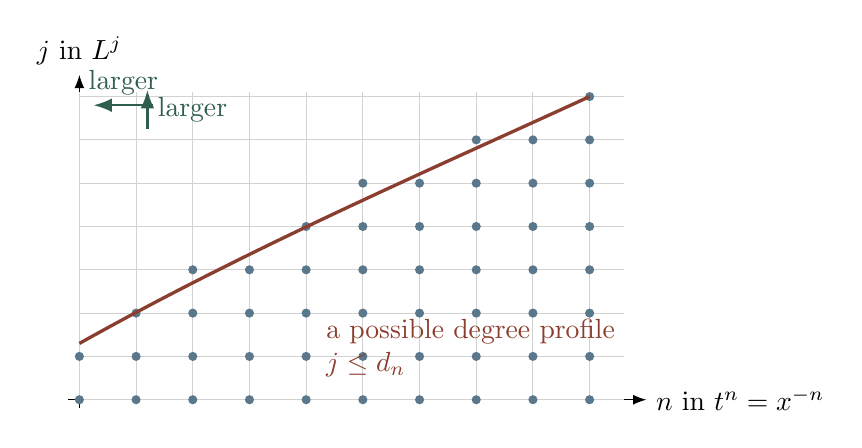
\begin{tikzpicture}[x=0.72cm,y=0.55cm,>=Latex]
  \draw[->] (-0.2,0)--(10.0,0) node[right] {$n$ in $t^n=x^{-n}$};
  \draw[->] (0,-0.2)--(0,7.5) node[above] {$j$ in $L^j$};
  \foreach \n in {0,...,9}{\draw[gray!35] (\n,0)--(\n,7.1);}
  \foreach \j in {0,...,7}{\draw[gray!35] (0,\j)--(9.6,\j);}
  \foreach \n/\d in {0/1,1/2,2/3,3/3,4/4,5/5,6/5,7/6,8/6,9/7}{
    \foreach \j in {0,...,\d}{\fill[DeepBlue!75] (\n,\j) circle (1.65pt);}
  }
  \draw[very thick,Brick] (0,1.3).. controls (3,3.5) and (6,5.2)..(9,7.0);
  \node[Brick,align=left] at (6.9,1.2) {a possible degree profile\\$j\le d_n$};
  \draw[->,thick,DeepGreen] (1.3,6.8)--(0.25,6.8) node[midway,above] {larger};
  \draw[->,thick,DeepGreen] (1.2,6.25)--(1.2,7.15) node[midway,right] {larger};
\end{tikzpicture}
\caption{A polynomial-logarithmic support.  Moving left increases the power of \(x\); at fixed \(n\), moving upward increases the logarithmic power.  Every vertical slice is finite.}
\label{fig:support-lattice}
\end{figure}

\subsection{Order, leading block, and leading monomial}

For nonzero \(F=\sum_{n\ge n_0}p_n(L)t^n\in\PLL\), define
\begin{equation}\label{eq:t-order}
 \ordt F\DefinitionEquals\min\SetOf{n:p_n\ne0},
\end{equation}
and adopt the usual convention \(\ordt 0=+\infty\).
The corresponding \emph{leading block} is \(t^{n_0}p_{n_0}(L)\).  If
\(d=\deg p_{n_0}\) and \(a\) is its leading coefficient, then
\begin{equation}\label{eq:leading-monomial}
 \lm(F)=t^{n_0}L^d=x^{-n_0}L^d,
 \qquad
 \lc(F)=a.
\end{equation}
The block valuation forgets the internal ordering in \(L\), but it is exactly the filtration needed for finite computation.

\begin{proposition}[Valuation laws]\label{prop:valuation-laws}
For nonzero \(F,G\in\PLL\),
\begin{align}
 \ordt(FG)&=\ordt F+\ordt G,\label{eq:ord-product}\\
 \ordt(F+G)&\ge\min(\ordt F,\ordt G),\label{eq:ord-sum}
\end{align}
with equality in \cref{eq:ord-sum} unless the leading blocks cancel.  At the refined monomial level,
\[
 \lm(FG)=\lm(F)\lm(G),\qquad \lc(FG)=\lc(F)\lc(G).
\]
\end{proposition}

\begin{proof}
Let the leading blocks be \(t^mp_m(L)\) and \(t^nQ_n(L)\).  The coefficient of \(t^{m+n}\) in the product is the nonzero polynomial \(p_mQ_n\), because \(\K[L]\) is an integral domain; no lower power of \(t\) can occur.  The assertion about leading monomials follows from the usual leading-term law for polynomial multiplication.  The sum law is immediate from coefficientwise addition.
\end{proof}

\subsection{\texorpdfstring{The \(t\)-adic filtration and truncation}{The t-adic filtration and truncation}}

For \(N\in\IntegerNumbers\), write
\begin{equation}\label{eq:formal-big-O}
 F=G+\FormalBigOAt{t^N}{t}
 \quad\Longleftrightarrow\quad
 F-G\in t^N\PL.
\end{equation}
This is a formal statement; it does not assert a uniform analytic bound in \(L\).  Define the truncation operator
\begin{equation}\label{eq:truncation}
 [F]_{<N}\DefinitionEquals\sum_{n<N}p_n(L)t^n.
\end{equation}
Then \(F=[F]_{<N}+\FormalBigOAt{t^N}{t}\).

\begin{proposition}[Completeness]\label{prop:complete}
The ring \(\PL\) is complete and separated for the filtration
\(\PL\supset t\PL\supset t^2\PL\supset\cdots\).  Equivalently, a sequence \(F_r\) converges if and only if, for every \(N\), the truncations \([F_r]_{<N}\) eventually stabilize.
\end{proposition}

\begin{proof}
This is the defining coefficientwise completeness of a formal power-series ring.  Stable coefficients \(p_0,\ldots,p_{N-1}\) for every \(N\) determine a unique series \(\sum_{n\ge0}p_nt^n\).  If an element lies in every \(t^N\PL\), all its coefficients vanish.
\end{proof}

This simple topology is the engine behind every infinite formula below.  A sum is legitimate whenever its contribution to each fixed power \(t^N\) is finite.  No numerical convergence is needed.

\subsection{Hahn-series viewpoint and general exponents}

For orientation, let
\[
 \mathfrak M_{\mathrm{pl}}=\SetOf{x^\alpha L^\beta:(\alpha,\beta)\in\RealNumbers^2}
\]
with lexicographic dominance.  A Hahn series with coefficients in \(\K\) and reverse-well-ordered support in this monomial group is a formal sum
\[
 \sum_{(\alpha,\beta)}c_{\alpha,\beta}x^\alpha L^\beta.
\]
The class \(\PLL\) embeds into this Hahn field.  Allowing arbitrary real \(\alpha\), or a well-ordered set of exponents, is useful for Puiseux-type inversions and differential equations.  We keep integer inverse powers in the main development because they make the coefficient algorithms transparent.  The proofs extend with little change to a well-ordered additive exponent semigroup, provided every target exponent has only finitely many decompositions relevant to a product.

\section{Multiplication: convolution of polynomial blocks}
\label{sec:multiplication}

\subsection{The Cauchy product}

Let
\begin{equation}\label{eq:F-G-series}
 F=\sum_{n\ge m}p_n(L)t^n,
 \qquad
 G=\sum_{n\ge r}Q_n(L)t^n.
\end{equation}
Their product is
\begin{equation}\label{eq:Cauchy-product}
 FG=\sum_{N\ge m+r}R_N(L)t^N,
 \qquad
 R_N(L)=\sum_{i+j=N}p_i(L)Q_j(L).
\end{equation}
For fixed \(N\), only finitely many pairs \((i,j)\) occur because both index sets are bounded below.  Thus the formal product is unambiguous even when neither series converges analytically.  This is the elementary special case of well-based transseries multiplication described by Edgar \cite{edgar-beginners}.

At the scalar-coefficient level, if
\[
 p_i(L)=\sum_a p_{i,a}L^a,
 \qquad
 Q_j(L)=\sum_b q_{j,b}L^b,
\]
then
\begin{equation}\label{eq:2d-convolution}
 [t^NL^d](FG)
 =\sum_{\substack{i+j=N\\a+b=d}}p_{i,a}q_{j,b}.
\end{equation}
Multiplication is therefore a two-dimensional convolution, with a finite vertical direction in every inverse-power block.

\begin{proposition}[Degree-profile bound]\label{prop:degree-profile}
Let \(d_i=\deg p_i\) and \(e_j=\deg Q_j\), with the degree of the zero polynomial taken as \(-\infty\).  Then
\begin{equation}\label{eq:degree-bound}
 \deg R_N\le\max_{i+j=N}(d_i+e_j).
\end{equation}
Equality holds unless the highest-degree contributions cancel.
\end{proposition}

\begin{proof}
Each product \(p_iQ_j\) has degree \(d_i+e_j\).  The degree of their finite sum cannot exceed the maximum.  Equality fails exactly when the sum of the leading coefficients over the maximizing pairs is zero.
\end{proof}

\subsection{Support geometry}

The support of a product lies in the Minkowski sum
\begin{equation}\label{eq:support-Minkowski}
 \CoefficientSupportOf{FG}\subseteq
 \CoefficientSupportOf{F}+\CoefficientSupportOf{G}.
\end{equation}
This viewpoint is especially useful when the allowed support occupies a cone or a staircase.  For example, for

\[
 F=\sum_{n\ge0}p_n(L)t^n,
 \qquad
 G=\sum_{n\ge0}Q_n(L)t^n,
\]
if \(a,c\ge0\) and
\[
 \deg p_n\le an+b,
 \qquad
 \deg Q_n\le cn+d,
\]
then
\begin{equation}\label{eq:linear-degree-profile}
 \deg R_N\le \max_{i+j=N}(ai+b+cj+d)
 \le \max(a,c)N+b+d.
\end{equation}
For Lambert's expansion, \(\deg \LambertPolynomial{n}=n\); products of finitely many such series therefore retain at most linear logarithmic-degree growth.

\subsection{A worked multiplication}

Consider
\begin{align*}
 F&=1+(L+1)t+(L^2-2L)t^2+(3-L)t^3+\FormalBigOAt{t^4}{t},\\
 G&=2-Lt+(L^2+1)t^2+2Lt^3+\FormalBigOAt{t^4}{t}.
\end{align*}
Using \cref{eq:Cauchy-product},
\begin{align*}
 R_0&=2,\\
 R_1&=2(L+1)-L=L+2,\\
 R_2&=2(L^2-2L)-(L+1)L+(L^2+1)
      =2L^2-5L+1,\\
 R_3&=2(3-L)-(L^2-2L)L+(L+1)(L^2+1)+2L\\
    &=3L^2+L+7.
\end{align*}
Hence
\begin{equation}\label{eq:worked-product}
 FG=2+(L+2)t+(2L^2-5L+1)t^2+(3L^2+L+7)t^3+\FormalBigOAt{t^4}{t}.
\end{equation}
Every coefficient calculation takes place in the ordinary polynomial ring \(\K[L]\).

\subsection{Truncation laws}

If \(F,G\in\PL\), then
\begin{equation}\label{eq:truncated-product-law}
 [FG]_{<N}=\bigl[[F]_{<N}[G]_{<N}\bigr]_{<N}.
\end{equation}
More generally, if \(\ordt F=m\) and \(\ordt G=r\), only coefficients of \(F\) below \(N-r\) and of \(G\) below \(N-m\) can contribute to a product modulo \(t^N\).  This precision bookkeeping is trivial but indispensable in symbolic implementations.

\begin{algorithmbox}[Naive truncated multiplication]
Given coefficient arrays \(p_m,\ldots,p_{N-1}\) and
\(Q_r,\ldots,Q_{N-1}\), initialize \(R_k=0\).  For every
\(i,j\) with \(i+j<N\), add the polynomial product \(p_iQ_j\) to
\(R_{i+j}\).  The algorithm uses \(\BigO(N^2)\) coefficient-ring
multiplications in the dense case; FFT or other fast convolution methods may be used when the truncation order is large.
\end{algorithmbox}

\section{Units, reciprocal series, and division}
\label{sec:division}

\subsection{Exactly which elements are invertible?}

\begin{theorem}[Units of \(\PL\)]\label{thm:units-P}
Let
\[
 F=p_0(L)+p_1(L)t+p_2(L)t^2+\cdots\in\PL.
\]
Then \(F\) is a unit of \(\PL\) if and only if \(p_0(L)\) is a nonzero constant in \(\K\).
\end{theorem}

\begin{proof}
A formal power series over a commutative ring is invertible exactly when its constant coefficient is invertible in the coefficient ring.  The only units of \(\K[L]\) are the nonzero constants.  For completeness, if \(FG=1\), the constant coefficient gives \(p_0Q_0=1\), so \(p_0\in\K^\times\).  Conversely, if \(p_0\in\K^\times\), the recurrence in \cref{thm:reciprocal-recurrence} constructs a unique reciprocal.
\end{proof}

\begin{corollary}[Units of the Laurent ring]\label{cor:units-Laurent}
A nonzero \(F\in\PLL\) is invertible in \(\PLL\) if and only if its leading block is
\(ct^m\) with \(c\in\K^\times\).  A leading factor \(P(L)t^m\) with nonconstant \(P\) is invertible in \(\QPL\), but generally not in \(\PLL\).
\end{corollary}

This distinction is often hidden by informal asymptotic notation.  Factoring the dominant monomial is not enough: one must ask whether its logarithmic coefficient is a unit in the chosen coefficient ring.

\subsection{Coefficient recurrence for reciprocals}

\begin{theorem}[Reciprocal recurrence]\label{thm:reciprocal-recurrence}
Let
\begin{equation}\label{eq:B-and-C}
 B=\sum_{n\ge0}Q_n(L)t^n,
 \qquad Q_0\in\K^\times.
\end{equation}
The unique reciprocal
\(C=B^{-1}=\sum_{n\ge0}C_n(L)t^n\) is determined by
\begin{align}
 C_0&=Q_0^{-1},\label{eq:reciprocal-C0}\\
 C_n&=-Q_0^{-1}\sum_{j=1}^{n}Q_jC_{n-j}
 \qquad(n\ge1).\label{eq:reciprocal-Cn}
\end{align}
All \(C_n\) are polynomials in \(L\).
\end{theorem}

\begin{proof}
Equating the coefficient of \(t^n\) in \(BC=1\) gives
\[
 \sum_{j=0}^{n}Q_jC_{n-j}=\begin{cases}1,&n=0,\\0,&n\ge1.\end{cases}
\]
The \(j=0\) term is \(Q_0C_n\); solve for \(C_n\).  Induction keeps every coefficient in \(\K[L]\).
\end{proof}

For a quotient \(A/B=R\), where
\(A=\sum p_nt^n\) and \(Q_0\in\K^\times\), the equivalent direct recurrence is
\begin{equation}\label{eq:quotient-recurrence}
 R_n=Q_0^{-1}\left(p_n-\sum_{j=1}^{n}Q_jR_{n-j}\right).
\end{equation}
This avoids first constructing all coefficients of \(B^{-1}\), although algebraically the two procedures are identical.

\subsection{A reciprocal example}

Let
\begin{equation}\label{eq:reciprocal-example-B}
 B=1+Lt+(L^2-1)t^2.
\end{equation}
The recurrence gives
\begin{align*}
 C_0&=1,\\
 C_1&=-L,\\
 C_2&=-\bigl(LC_1+(L^2-1)C_0\bigr)=1,\\
 C_3&=-\bigl(LC_2+(L^2-1)C_1\bigr)=L^3-2L,\\
 C_4&=-\bigl(LC_3+(L^2-1)C_2\bigr)=-L^4+L^2+1.
\end{align*}
Thus
\begin{equation}\label{eq:reciprocal-example-C}
 \frac1B=1-Lt+t^2+(L^3-2L)t^3+(-L^4+L^2+1)t^4+\FormalBigOAt{t^5}{t}.
\end{equation}
A direct multiplication verifies that the product of
\cref{eq:reciprocal-example-B,eq:reciprocal-example-C} is
\(1+\FormalBigOAt{t^5}{t}\).

\subsection{Geometric-series factorization}

If \(B=c(1+U)\) with \(c\in\K^\times\) and \(U\in t\PL\), then
\begin{equation}\label{eq:geometric-reciprocal}
 B^{-1}=c^{-1}\sum_{k=0}^{\infty}(-U)^k.
\end{equation}
The sum is \(t\)-adically well defined because \(U^k\in t^k\PL\).  Formula \cref{eq:geometric-reciprocal} is conceptually useful; the coefficient recurrence is usually more efficient.

If the leading coefficient is a nonconstant polynomial \(Q_0(L)\), the same factorization works in \(\QPL\):
\begin{equation}\label{eq:rational-leading-reciprocal}
 B^{-1}=Q_0(L)^{-1}
 \left(1+\frac{B-Q_0}{Q_0}\right)^{-1}.
\end{equation}
Every coefficient is then rational in \(L\).  For example,
\begin{equation}\label{eq:nonclosure-example}
 \frac1{L+1+t}
 =\frac1{L+1}-\frac{t}{(L+1)^2}
 +\frac{t^2}{(L+1)^3}-\cdots.
\end{equation}
No rearrangement turns these coefficients into polynomials in \(L\).

\subsection{Newton iteration for reciprocal}

Suppose \(C\) approximates \(B^{-1}\).  Newton's iteration for the equation
\(C^{-1}-B=0\) takes the familiar form
\begin{equation}\label{eq:newton-reciprocal}
 C_{\mathrm{new}}=C(2-BC).
\end{equation}
If
\(BC=1+E\) with \(E\in t^N\PL\), then
\begin{equation}\label{eq:newton-reciprocal-error}
 BC_{\mathrm{new}}=(1+E)(1-E)=1-E^2
 =1+\FormalBigOAt{t^{2N}}{t}.
\end{equation}
Thus each step doubles the number of correct inverse-power blocks.  Starting from \(C_0=Q_0^{-1}\), one computes modulo \(t,t^2,t^4,t^8,\ldots\).  With fast multiplication this is asymptotically superior to the quadratic recurrence.

\subsection{Powers, logarithms, and exponentials of small series}

The same completeness argument defines the standard formal functions.  For
\(U\in t\PL\) and \(\alpha\in\K\),
\begin{align}
 (1+U)^\alpha
 &=\sum_{k=0}^{\infty}\binom{\alpha}{k}U^k,
 \label{eq:binomial-small}\\
 \log(1+U)
 &=\sum_{k=1}^{\infty}\frac{(-1)^{k+1}}{k}U^k,
 \label{eq:log-small}\\
 \exp(U)
 &=\sum_{k=0}^{\infty}\frac{U^k}{k!}.
 \label{eq:exp-small}
\end{align}
Each coefficient of \(t^N\) receives contributions only from \(k\le N\).  Therefore these are exact formal identities in \(\PL\), not heuristic Taylor substitutions.

For a general unit \(B=c(1+U)\), one may set
\[
 \log B=\log c+\log(1+U)
\]
after choosing a logarithm of \(c\).  For nonconstant leading \(Q_0(L)\), \(\log Q_0(L)\) is usually not polynomial in \(L\); one again leaves the one-logarithm coefficient ring.

\begin{keybox}[Algebraic closure summary]
\begin{center}
\begin{tabular}{@{}lll@{}}
\toprule
Operation & Sufficient hypothesis & Resulting class\\
\midrule
addition, multiplication & none & \(\PL\)\\
reciprocal & constant nonzero leading coefficient & \(\PL\)\\
reciprocal & nonzero polynomial leading coefficient & \(\K(L)((t))\)\\
\((1+U)^\alpha,\log(1+U),\exp U\) & \(U\in t\PL\) & \(\PL\)\\
\bottomrule
\end{tabular}
\end{center}
\end{keybox}

\section{Differential and integral calculus}
\label{sec:differential-calculus}

The variables \(t=x^{-1}\) and \(L=\log x\) satisfy
\begin{equation}\label{eq:t-L-derivatives}
 \frac{\Differential t}{\Differential x}=-t^2,
 \qquad
 \frac{\Differential L}{\Differential x}=t.
\end{equation}
Consequently the derivation induced by the relation between them is
\begin{equation}\label{eq:D-operator}
 \D=t\partial_L-t^2\partial_t.
\end{equation}
This is not the partial derivative with respect to either formal variable separately.

\subsection{Differentiating a block}

For a block \(t^nP(L)\),
\begin{equation}\label{eq:block-derivative}
 \D\bigl(t^nP(L)\bigr)
 =t^{n+1}\bigl(P'(L)-nP(L)\bigr).
\end{equation}
It is convenient to introduce the shifted differential operator
\begin{equation}\label{eq:Delta-n}
 \Delta_n\DefinitionEquals\partial_L-n.
\end{equation}
Then
\begin{equation}\label{eq:block-derivative-Delta}
 \D\bigl(t^nP(L)\bigr)=t^{n+1}\Delta_nP(L).
\end{equation}
Repeated differentiation shifts the index at each step.

\begin{proposition}[Higher derivatives]\label{prop:higher-derivative}
For \(k\ge0\),
\begin{equation}\label{eq:higher-derivative}
 \D^k\bigl(t^nP(L)\bigr)
 =t^{n+k}
 \prod_{j=0}^{k-1}\bigl(\partial_L-(n+j)\bigr)P(L),
\end{equation}
where the empty product for \(k=0\) is the identity.
\end{proposition}

\begin{proof}
The case \(k=1\) is \cref{eq:block-derivative}.  If the formula holds for \(k\), apply \(\D\) once more.  The current power of \(t\) is \(n+k\), so \cref{eq:block-derivative-Delta} adds the factor
\(\partial_L-(n+k)\) and one further power of \(t\).
\end{proof}

\begin{corollary}[Continuity of differentiation]\label{cor:D-continuous}
For \(F\in\PLL\),
\begin{equation}\label{eq:D-order}
 \ordt(\D F)\ge\ordt F+1,
\end{equation}
with strict inequality possible only when the leading coefficient polynomial lies in the kernel of the relevant \(\Delta_n\).  In particular, \(\D\) is continuous in the \(t\)-adic topology.
\end{corollary}

For polynomial coefficients the kernel issue is simple.  If \(n\ne0\), the equation \(P'-nP=0\) has no nonzero polynomial solution; if \(n=0\), constants are killed.  Thus differentiation raises the block order by exactly one except for a constant leading block.

\subsection{Integration remains polynomial-logarithmic}

To integrate \(t^nP(L)\), seek an antiderivative of the form
\(t^{n-1}Q(L)\).  Equation \cref{eq:block-derivative} becomes
\begin{equation}\label{eq:antiderivative-equation}
 Q'(L)-(n-1)Q(L)=P(L).
\end{equation}
If \(n=1\), this is simply \(Q'=P\), so any polynomial antiderivative works.  If \(n\ne1\), the operator
\(\partial_L-(n-1)\) is invertible on \(\K[L]\), and its inverse is finite because sufficiently high derivatives of a polynomial vanish:
\begin{equation}\label{eq:Delta-inverse-polynomial}
 Q(L)=-\sum_{j=0}^{\deg P}
 \frac{P^{(j)}(L)}{(n-1)^{j+1}}.
\end{equation}
A direct telescoping calculation verifies
\((\partial_L-(n-1))Q=P\).

\begin{proposition}[Formal antiderivatives]\label{prop:formal-antiderivatives}
Every element of \(\PLL\) has a termwise antiderivative in \(\PLL\), unique up to an additive constant.
\end{proposition}

\begin{proof}
Apply the preceding construction to every block.  A target coefficient at \(t^N\) receives a contribution from exactly one source block, so the termwise sum is well defined.  The only kernel of \(\D\) in \(\PLL\) is \(\K\): take a nonconstant series, inspect its leading block, and use the kernel observation following \cref{cor:D-continuous}.
\end{proof}

The result is stronger than one might expect from elementary integration tables.  The obstruction \(\int \Differential x/(x\log x)=\log\log x\) does not contradict it, because \(1/(x\log x)=t/L\) is already outside \(\PLL\).  Once rational or negative logarithmic powers are admitted, new logarithmic levels can indeed be forced.

\subsection{Differential operators on coefficient polynomials}

Many calculations can be performed without expanding every monomial.  Define
\begin{equation}\label{eq:falling-D-operator}
 (\partial_L-n)_{k}^{\downarrow}
 \DefinitionEquals\prod_{j=0}^{k-1}(\partial_L-n-j).
\end{equation}
Then
\[
 \D^k(t^nP)=t^{n+k}(\partial_L-n)_{k}^{\downarrow}P.
\]
The operators are polynomials in \(\partial_L\), hence commute.  This observation gives a compact shifted-Taylor notation for composition and makes Lagrange reversion particularly compact.

\section{Composition with a near-identity inner transseries}
\label{sec:composition}

Composition is the first operation for which the relation \(L=\log x\) is essential.  It is also the operation whose domain conditions matter most in full transseries theory \cite{edgar-composition,vanderhoeven-book}.  In the one-logarithm class, a clean and useful domain is provided by inner series asymptotic to \(x\).

\subsection{The near-identity group candidate}

Define
\begin{equation}\label{eq:Gnear-def}
 \Gnear\DefinitionEqualsx+\PL
 =\SetOf{x+A(x):A\in\K[L][[x^{-1}]]}.
\end{equation}
Every \(G=x+A\in\Gnear\) can be factored as
\begin{equation}\label{eq:G-factor}
 G=x(1+u),
 \qquad
 u=tA\in t\PL.
\end{equation}
Thus \(G/x=1+u\) is a unit infinitesimally close to \(1\).  Formally and analytically, every polynomial in \(\log x\) is smaller than \(x\), so allowing an arbitrary \(t^0\) polynomial block in \(A\) is harmless.

Set
\begin{equation}\label{eq:lambda-def}
 \lambda\DefinitionEquals\log(1+u)\in t\PL.
\end{equation}
Then
\begin{equation}\label{eq:logG-and-inverseG}
 \log G=L+\lambda,
 \qquad
 G^{-n}=t^n(1+u)^{-n}=t^n\EulerE^{-n\lambda}.
\end{equation}

\subsection{Exact substitution formula}

Let
\begin{equation}\label{eq:F-general-composition}
 F(x)=\sum_{n\ge n_0}t^np_n(L)\in\PLL,
 \qquad
 G=x+A\in\Gnear.
\end{equation}
The natural substitution is
\begin{equation}\label{eq:composition-master}
 (F\compose G)(x)
 =\sum_{n\ge n_0}t^n(1+u)^{-n}
 p_n\bigl(L+\lambda\bigr),
\end{equation}
where \(u=tA\) and \(\lambda=\log(1+u)\).

\begin{theorem}[Closure under near-identity composition]\label{thm:composition-closure}
Formula \cref{eq:composition-master} defines a unique element of \(\PLL\).  If \(F\in\PL\), then \(F\compose G\in\PL\).  For every \(N\), its truncation modulo \(t^N\) depends on only finitely many coefficients of \(F\) and \(G\).
\end{theorem}

\begin{proof}
Because \(u,\lambda\in t\PL\), the binomial series for \((1+u)^{-n}\) and the powers of \(\lambda\) are \(t\)-adically defined.  Since \(p_n\) is a polynomial,
\begin{equation}\label{eq:polynomial-shift}
 p_n(L+\lambda)
 =\sum_{j=0}^{\deg p_n}\frac{p_n^{(j)}(L)}{j!}\lambda^j
\end{equation}
contains only finitely many Taylor terms.  For a fixed target power \(t^N\), only indices \(n_0\le n\le N\) can contribute, and for each such \(n\) only finitely many terms of the binomial and logarithmic series are needed.  All resulting coefficients are polynomials in \(L\).
\end{proof}

The formula admits a compact \emph{shifted-Taylor} notation.  Recall
\(\Delta_n=\partial_L-n\), and define, for \(P\in\K[L]\),
\begin{equation}\label{eq:normal-shift-operator}
 \mathcal E_{\lambda,n}P
 \DefinitionEquals\sum_{k=0}^{\infty}\frac{\lambda^k}{k!}\Delta_n^kP.
\end{equation}
Here every \(\Delta_n^k\) acts on \(P\) \emph{before} multiplication by
\(\lambda^k\).  The binomial theorem gives the exact identity
\begin{align}
 \EulerE^{-n\lambda}P(L+\lambda)
 &=\left(\sum_{a\ge0}\frac{(-n\lambda)^a}{a!}\right)
   \left(\sum_{b\ge0}\frac{\lambda^b}{b!}P^{(b)}(L)\right)\notag\\
 &=\sum_{k\ge0}\frac{\lambda^k}{k!}(\partial_L-n)^kP(L)
 =\mathcal E_{\lambda,n}P.\label{eq:shifted-Taylor-identity}
\end{align}
Consequently
\begin{equation}\label{eq:composition-operator-form}
 F\compose G
 =\sum_{n\ge n_0}t^n\mathcal E_{\lambda,n}p_n(L).
\end{equation}
For a nonzero polynomial \(P\), the sum over \(k\) in
\cref{eq:normal-shift-operator} generally terminates only when \(n=0\),
but every coefficient of \(t^N\) receives finitely many
contributions because \(\lambda\in t\PL\).

\begin{warningbox}[Normal ordering is essential]
One may write \(\mathcal E_{\lambda,n}\) suggestively as
\(\mathopen{:}\!\exp(\lambda\Delta_n)\!\mathclose{:}\), with the colons
meaning that all powers of \(\lambda\) are placed to the left of all
\(\Delta_n\)'s.  It is generally \emph{not} the ordinary operator
exponential \(\exp(M_\lambda\Delta_n)\), where \(M_\lambda\) denotes
multiplication by \(\lambda\): ordinary iteration would let
\(\partial_L\) differentiate \(\lambda(t,L)\).  The two coincide only
when \(\partial_L\lambda=0\).  This distinction is easy to miss in
polynomial-logarithmic composition.
\end{warningbox}

\subsection{Taylor's formula at infinity}

There is an equivalent expression that looks exactly like ordinary Taylor expansion.

\begin{theorem}[Formal Taylor composition]\label{thm:formal-Taylor}
For \(F\in\PLL\) and \(A\in\PL\),
\begin{equation}\label{eq:formal-Taylor}
 F(x+A)=\sum_{k=0}^{\infty}\frac{A(x)^k}{k!}\D^kF(x)
\end{equation}
is a well-defined \(t\)-adic sum and equals \cref{eq:composition-master}.
\end{theorem}

\begin{proof}
Consider first one block \(F=t^nP(L)\).  By
\cref{prop:higher-derivative}, \(\D^kF\in t^{n+k}\PL\).  Since
\(A^k\in\PL\), the \(k\)-th summand has order at least \(n+k\), so only finitely many \(k\) affect any prescribed truncation.  The same remains true after summing over \(n\), which is bounded below.

To identify the sum, temporarily insert a scalar parameter \(s\) and consider
\(H(s)=F(x+sA(x))\), treating \(A(x)\) as constant with respect to \(s\).  Formal differentiation in \(s\) gives
\(H^{(k)}(0)=A^k\D^kF(x)\).  The resulting formal Taylor series in \(s\), evaluated at \(s=1\), produces \cref{eq:formal-Taylor}.  Direct substitution of
\(x+A=x(1+u)\) gives \cref{eq:composition-master}; both expressions agree coefficientwise.
\end{proof}

\begin{remark}
The smallness condition is relative: \(A\) need not tend to zero.  It may be \(L^{100}\), for example.  What matters is \(A/x=tA\in t\PL\), so each differentiation in \cref{eq:formal-Taylor} gains an inverse power of \(x\).
\end{remark}

\subsection{Low-order composition coefficients}

Let
\begin{align}
 F&=x+A_0(L)+A_1(L)t+A_2(L)t^2+A_3(L)t^3+\FormalBigOAt{t^4}{t},
 \label{eq:F-near-low}\\
 G&=x+B_0(L)+B_1(L)t+B_2(L)t^2+B_3(L)t^3+\FormalBigOAt{t^4}{t},
 \label{eq:G-near-low}
\end{align}
and write
\begin{equation}\label{eq:H-near-low}
 F\compose G=x+C_0(L)+C_1(L)t+C_2(L)t^2+C_3(L)t^3+\FormalBigOAt{t^4}{t}.
\end{equation}
Primes below denote \(\Differential/\Differential L\).  Expanding either
\cref{eq:composition-master} or \cref{eq:formal-Taylor} gives
\begin{align}
 C_0={}&B_0+A_0,\label{eq:C0-compose}\\
 C_1={}&B_1+A_1+B_0A_0',\label{eq:C1-compose}\\
 C_2={}&B_2+A_2+B_0(A_1'-A_1)+B_1A_0'
 +\frac{B_0^2}{2}(A_0''-A_0'),\label{eq:C2-compose}\\
 C_3={}&B_3+A_3+B_0(A_2'-2A_2)+B_1(A_1'-A_1)+B_2A_0'
 \notag\\
 &+\frac{B_0^2}{2}(A_1''-3A_1'+2A_1)
 +B_0B_1(A_0''-A_0')\notag\\
 &+\frac{B_0^3}{6}(A_0'''-3A_0''+2A_0').
 \label{eq:C3-compose}
\end{align}
These formulas display three sources of terms: direct coefficients of \(F\) and \(G\), translation of \(L\), and rescaling of inverse powers by \(G^{-n}\).

\subsection{Coefficient recurrences for efficient composition}

Suppose
\begin{equation}\label{eq:lambda-coefficients}
 \lambda(t,L)=\sum_{j\ge1}\lambda_j(L)t^j.
\end{equation}
For a fixed outer block \(p_n\), define
\begin{equation}\label{eq:E-n-r-def}
 E_n(t,L)\DefinitionEquals\EulerE^{-n\lambda(t,L)}p_n\bigl(L+\lambda(t,L)\bigr)
 =\sum_{r\ge0}E_{n,r}(L)t^r.
\end{equation}
There are two useful exact recurrences.

First set
\begin{equation}\label{eq:rho-composition}
 \rho(t,L)\DefinitionEquals\frac{\partial_t\lambda}{1+\partial_L\lambda}
 =\sum_{q\ge0}\rho_q(L)t^q.
\end{equation}
The denominator is a unit because \(\partial_L\lambda\in t\PL\).  Direct
differentiation of \cref{eq:E-n-r-def} gives
\begin{equation}\label{eq:E-PDE}
 \partial_tE_n=\rho\,\Delta_nE_n.
\end{equation}
Indeed,
\[
 \partial_tE_n=\lambda_t\EulerE^{-n\lambda}
 \bigl(p_n'-np_n\bigr)(L+\lambda),
\]
whereas
\[
 \Delta_nE_n=(1+\lambda_L)\EulerE^{-n\lambda}
 \bigl(p_n'-np_n\bigr)(L+\lambda).
\]
Comparing coefficients of \(t\) in \cref{eq:E-PDE} yields
\begin{align}
 E_{n,0}&=p_n,\label{eq:E-rec-0}\\
 rE_{n,r}&=\sum_{q=0}^{r-1}\rho_q\,\Delta_nE_{n,r-1-q}
 \qquad(r\ge1).\label{eq:E-rec-r}
\end{align}
Unlike the tempting but incorrect replacement
\(\rho=\partial_t\lambda\), this recurrence automatically accounts for
the \(L\)-dependence of the logarithmic shift.

A second method avoids differentiating already-computed coefficients.  Define
\begin{equation}\label{eq:b-r-k-def}
 \frac{\lambda^k}{k!}=\sum_{r\ge k}b_{r,k}(L)t^r.
\end{equation}
Then
\begin{align}
 b_{0,0}&=1,\qquad b_{r,0}=0\quad(r>0),\label{eq:b-boundary}\\
 b_{r,k}&=\frac1k\sum_{j=1}^{r-k+1}
 \lambda_jb_{r-j,k-1}
 \qquad(1\le k\le r),\label{eq:b-recurrence}\\
 E_{n,r}&=\sum_{k=0}^{r}b_{r,k}\Delta_n^kp_n.\label{eq:E-from-b}
\end{align}
Equivalently, in terms of the partial exponential Bell polynomials,
\begin{equation}\label{eq:Bell-operator-composition}
 E_{n,r}=\frac1{r!}\sum_{k=0}^{r}
 B_{r,k}\bigl(1!\lambda_1,2!\lambda_2,\ldots,
 (r-k+1)!\lambda_{r-k+1}\bigr)\Delta_n^kp_n.
\end{equation}
Here \(B_{0,0}=1\), while \(B_{r,0}=0\) for \(r>0\).
In \cref{eq:Bell-operator-composition}, the Bell-polynomial coefficient
is formed first and only then multiplied by \(\Delta_n^kp_n\); no
differential operator acts on the \(\lambda_j\)'s.  Finally,
\begin{equation}\label{eq:compose-from-E}
 [t^N](F\compose G)=\sum_{n=n_0}^{N}E_{n,N-n}.
\end{equation}
The \(\rho\)-recurrence is convenient when polynomial differentiation is
cheap; the \(b_{r,k}\)-recurrence is convenient when the shifted
derivatives \(\Delta_n^kp_n\) can be cached.

\subsection{Associativity and the identity}

Substitution into actual expressions is associative whenever all compositions are defined.  The formal construction retains this property.

\begin{proposition}[Associativity in the near-identity domain]\label{prop:composition-associative}
If \(F\in\PLL\) and \(G,H\in\Gnear\), then
\begin{equation}\label{eq:composition-assoc}
 (F\compose G)\compose H=F\compose(G\compose H).
\end{equation}
Moreover, \(x\) is a two-sided identity and \(G\compose H\in\Gnear\).
\end{proposition}

\begin{proof}
Introduce finite truncations modulo \(t^N\).  Every coefficient on either side is obtained from a finite polynomial-rational calculation in the finitely many input coefficients, for which ordinary substitution is associative.  Since the truncations agree for every \(N\), the formal series agree.  Closure follows from \cref{thm:composition-closure} applied to the correction part of \(G\).
\end{proof}

\subsection{Where composition leaves the class}

Near-identity composition is not an arbitrary technical restriction; it marks a genuine closure boundary.

\paragraph{Constant dilations.}
For \(G=ax\), with a chosen logarithm of \(a\),
\[
 t\mapsto a^{-1}t,
 \qquad
 L\mapsto L+\log a,
\]
so polynomial-logarithmic series remain polynomial-logarithmic.

\paragraph{Power substitutions.}
For \(G=x^\rho\),
\[
 t^n\mapsto x^{-\rho n},
 \qquad
 L\mapsto\rho L.
\]
The class remains one-logarithmic but generally requires noninteger exponents.

\paragraph{Logarithmic factors in the leading monomial.}
For
\(G=x^\rho L^\sigma(1+u)\),
\begin{equation}\label{eq:log-leading-log-factor}
 \log G=\rho L+\sigma\log L+\log(1+u).
\end{equation}
If \(\sigma\ne0\), the new symbol \(\log L=\log\log x\) is unavoidable.  One must pass to a two-logarithm class.

\paragraph{Exponential changes of scale.}
If \(G=\EulerE^x\), then inverse powers of \(G\) become exponentially small monomials \(\EulerE^{-nx}\), and \(\log G=x\).  Such substitutions belong naturally to the full logarithmic-exponential transseries field, not to \(\PLL\).

\begin{warningbox}[Composition is directional]
The fact that \(F\compose G\) is defined and remains in a chosen class says nothing automatic about \(G\compose F\).  The outer series determines which functions of the inner leading scale must be formed.  Full transseries composition therefore comes with explicit domain conditions, typically requiring the inner argument to be positive and infinitely large; see \cite{edgar-composition,vanderhoeven-book}.
\end{warningbox}

\section{Series reversal: compositional inversion at infinity}
\label{sec:reversion}

\subsection{The triangular structure}

Let
\begin{equation}\label{eq:F-reversion}
 F=x+A,
 \qquad A\in\PL.
\end{equation}
We seek
\begin{equation}\label{eq:G-reversion}
 G=x+B,
 \qquad B\in\PL,
\end{equation}
such that \(F\compose G=x\).  The coefficient equations are triangular because changing the \(t^N\) block of \(G\) changes the \(t^N\) block of \(F\compose G\) by exactly the same amount to first order.

\begin{lemma}[Triangular perturbation]\label{lem:triangular-perturbation}
Let \(F=x+A\in\Gnear\), \(G\in\Gnear\), and \(c(L)\in\K[L]\).  Then
\begin{equation}\label{eq:triangular-perturbation}
 F\compose\bigl(G+c(L)t^N\bigr)
 =F\compose G+c(L)t^N+\FormalBigOAt{t^{N+1}}{t}.
\end{equation}
\end{lemma}

\begin{proof}
Apply formal Taylor expansion to the outer series \(F\) at \(G\):
\[
 F(G+\delta)=F(G)+F'(G)\delta+\frac12F''(G)\delta^2+\cdots,
 \qquad \delta=c(L)t^N.
\]
Since \(F'=1+\FormalBigOAt{t}{t}\), the linear term is
\(c(L)t^N+\FormalBigOAt{t^{N+1}}{t}\).  Also \(F''=\FormalBigOAt{t^2}{t}\), so every term of degree at least two in \(\delta\) has order greater than \(N\).
\end{proof}

\begin{theorem}[Existence and uniqueness of reversion]\label{thm:reversion-existence}
Every \(F\in\Gnear\) has a unique two-sided compositional inverse
\begin{equation}\label{eq:inverse-in-Gnear}
 F^{\rev}\in\Gnear.
\end{equation}
Consequently \(\Gnear\) is a group under composition.
\end{theorem}

\begin{proof}
Begin with \(G_{<0}=x\).  Suppose coefficients through \(t^{N-1}\) have been chosen so that
\begin{equation}\label{eq:reversion-residual-N}
 F\compose G_{<N}=x+r_N(L)t^N+\FormalBigOAt{t^{N+1}}{t}.
\end{equation}
By \cref{lem:triangular-perturbation}, replacing \(G_{<N}\) by
\[
 G_{<N+1}=G_{<N}-r_N(L)t^N
\]
cancels the residual block and preserves all lower blocks.  Induction and completeness produce a right inverse \(G\) with \(F\compose G=x\).

Apply the same construction to \(G\) and obtain \(H\in\Gnear\) with
\(G\compose H=x\).  Associativity now gives
\[
 F=F\compose(G\compose H)=(F\compose G)\compose H=H,
\]
so \(G\compose F=G\compose H=x\); hence \(G\) is two-sided.  Uniqueness follows from the same triangular leading-difference argument: if two right inverses first differ in their \(t^N\) blocks, their images under \(F\) differ in that block by \cref{lem:triangular-perturbation}, a contradiction.
\end{proof}

\subsection{Coefficient-by-coefficient reversion algorithm}

The proof is already an algorithm.

\begin{algorithm}[htbp]
\caption{Triangular reversion in \(\Gnear\)}
\label{alg:triangular-reversion}
\begin{algorithmic}[1]
\Require \(F=x+A\), target precision \(t^N\)
\State \(G\gets x\)
\For{\(n=0,1,\ldots,N-1\)}
  \State compute \(r_n(L)=[t^n](F\compose G-x)\)
  \State \(G\gets G-r_n(L)t^n\)
\EndFor
\State \Return \([G]_{<N}\)
\end{algorithmic}
\end{algorithm}

A naive implementation recomposes from scratch at every step.  Incremental use of \cref{eq:E-rec-r}, or Newton iteration below, is preferable at high order.

\subsection{Explicit low-order inverse coefficients}

Write
\begin{align}
 F={}&x+A_0+A_1t+A_2t^2+A_3t^3+\FormalBigOAt{t^4}{t},\label{eq:F-inverse-low}\\
 F^{\rev}={}&x+B_0+B_1t+B_2t^2+B_3t^3+\FormalBigOAt{t^4}{t}.
 \label{eq:G-inverse-low}
\end{align}
Setting \(C_0,C_1,C_2,C_3\) in
\cref{eq:C0-compose,eq:C1-compose,eq:C2-compose,eq:C3-compose} equal to zero gives
\begin{align}
 B_0={}&-A_0,\label{eq:B0-inverse}\\
 B_1={}&-A_1+A_0A_0',\label{eq:B1-inverse}\\
 B_2={}&-A_2+A_0(A_1'-A_1)+A_1A_0'
 -A_0(A_0')^2
 -\frac{A_0^2}{2}(A_0''-A_0').
 \label{eq:B2-inverse}
\end{align}
The next coefficient is already large enough to justify algorithmic generation:
\begin{align}
 B_3={}&-A_3-A_1^2+A_1A_1'+A_0'A_2-2A_0A_2+A_0A_2'
 \notag\\
 &-(A_0')^2A_1+3A_0A_0'A_1-2A_0A_0'A_1'-A_0A_0''A_1
 \notag\\
 &+A_0(A_0')^3-\frac32A_0^2(A_0')^2
 +\frac32A_0^2A_0'A_0''
 \notag\\
 &-A_0^2A_1+\frac32A_0^2A_1'-\frac12A_0^2A_1''
 \notag\\
 &+\frac13A_0^3A_0'-\frac12A_0^3A_0''
 +\frac16A_0^3A_0'''.
 \label{eq:B3-inverse}
\end{align}
Every derivative is with respect to \(L\).  These expressions are differential polynomials with rational coefficients in the input blocks.

\subsection{Newton reversion}

Let \(G\) be an approximate inverse and let
\begin{equation}\label{eq:reversion-residual}
 R=F\compose G-x.
\end{equation}
Linearizing in a correction \(\delta\) gives
\[
 F\compose(G+\delta)-x
 =R+(F'\compose G)\delta+\text{quadratic terms}.
\]
This suggests
\begin{equation}\label{eq:newton-reversion}
 G_{\mathrm{new}}
 =G-\frac{F\compose G-x}{F'\compose G}.
\end{equation}
The denominator is a unit because \(F'=1+\FormalBigOAt{t}{t}\).

\begin{proposition}[Precision improvement]\label{prop:newton-reversion-precision}
If \(F\compose G-x\in t^N\PL\), then the Newton update
\cref{eq:newton-reversion} satisfies
\begin{equation}\label{eq:newton-reversion-precision}
 F\compose G_{\mathrm{new}}-x\in t^{2N+2}\PL.
\end{equation}
In particular, the number of correct blocks at least doubles asymptotically.
\end{proposition}

\begin{proof}
Set \(\delta=-R/(F'\compose G)\).  Then \(\delta\in t^N\PL\), and the constant and linear terms in the Taylor expansion cancel.  Since \(F''\in t^2\PL\), the quadratic remainder begins in
\(t^{2N+2}\PL\); higher terms are still smaller.
\end{proof}

In practical code one truncates all intermediate products, compositions, and reciprocals to the target precision of the current Newton stage.

\subsection{Lagrange--B\"urmann reversion at infinity}

There is also a closed formal series for the inverse of \(F=x+\phi(x)\).  It is the additive form of the Lagrange--B\"urmann inversion theorem.

\begin{theorem}[Lagrange reversion formula]\label{thm:Lagrange-reversion}
For \(\phi\in\PL\), the inverse of
\begin{equation}\label{eq:F-x-plus-phi}
 F(x)=x+\phi(x)
\end{equation}
is
\begin{equation}\label{eq:Lagrange-reversion}
 F^{\rev}(y)
 =y+\sum_{k=1}^{\infty}\frac{(-1)^k}{k!}
 \left(\frac{\Differential}{\Differential y}\right)^{k-1}\!\bigl(\phi(y)^k\bigr).
\end{equation}
The sum is well defined in \(y+\K[\log y][[y^{-1}]]\).
\end{theorem}

\begin{proof}
Insert the labelled auxiliary parameter \(\LagrangeAuxiliaryParameter\) and solve
\[
 y=x+\LagrangeAuxiliaryParameter\phi(x),
 \qquad x=y+w.
\]
Then \(w=-\LagrangeAuxiliaryParameter\phi(y+w)\).  Ordinary formal Lagrange inversion in \(\LagrangeAuxiliaryParameter\) gives
\[
 w=\sum_{k\ge1}\frac{(-\LagrangeAuxiliaryParameter)^k}{k!}
 \left(\frac{\Differential}{\Differential y}\right)^{k-1}\phi(y)^k.
\]
For \(\phi\in\PL\), the \((k-1)\)-st derivative raises \(t\)-order by at least \(k-1\), so the coefficient of each fixed inverse power receives contributions from only finitely many \(k\).  Therefore setting \(\LagrangeAuxiliaryParameter=1\) is legitimate in the \(t\)-adic topology and yields \cref{eq:Lagrange-reversion}.
\end{proof}

\begin{remark}
Formula \cref{eq:Lagrange-reversion} is direct but not always computationally optimal: forming \(\phi^k\) and differentiating it separately repeats work.  It is nevertheless invaluable for proofs, for explicit coefficient formulas, and for recognizing combinatorial number triangles.
\end{remark}

\subsection{A perturbed logarithmic example}

Take
\begin{equation}\label{eq:perturbed-log-map}
 F(x)=x+\log x+\frac{c}{x}.
\end{equation}
Here \(A_0=L\), \(A_1=c\), and \(A_n=0\) for \(n\ge2\).  The low-order formulas give
\begin{align}
 F^{\rev}(x)={}&x-L+(L-c)t
 +\left(\frac{L^2}{2}-(c+1)L+c\right)t^2
 \notag\\
 &+\frac{1}{6}\left(2L^3-(6c+9)L^2+(18c+6)L-6c^2-6c\right)t^3
 +\FormalBigOAt{t^4}{t}.
 \label{eq:perturbed-log-inverse}
\end{align}
Substitution into \cref{eq:perturbed-log-map} cancels every block through \(t^3\).  The case \(c=0\) is the inverse of \(x+\log x\), to which we now turn.

\section{\texorpdfstring{The inverse of \(x+\log x\) and the Lambert polynomials}{The inverse of x + log x and the Lambert polynomials}}
\label{sec:Lambert-polynomials}

\subsection{The Wright omega equation}

For real \(x\) sufficiently large, let \(\WrightOmega(x)\) be the positive solution of
\begin{equation}\label{eq:omega-equation}
 \WrightOmega+\log\WrightOmega=x.
\end{equation}
Equivalently,
\begin{equation}\label{eq:omega-W}
 \WrightOmega(x)=\LambertW_0(\EulerE^x).
\end{equation}
Thus \(\WrightOmega\) is exactly the compositional inverse of
\begin{equation}\label{eq:F-log-map}
 F(y)=y+\log y.
\end{equation}
By \cref{thm:reversion-existence}, it has a unique formal expansion in \(\Gnear\).  We write it as
\begin{equation}\label{eq:omega-expansion}
 \WrightOmega(x)=x+\mathcal P(t,L)
 =x-L+\sum_{n=1}^{\infty}\LambertPolynomial{n}(L)t^n,
 \qquad t=x^{-1},\quad L=\log x,
\end{equation}
where, for convenience,
\begin{equation}\label{eq:P0-def}
 \LambertPolynomial{0}(L)\DefinitionEquals-L,
 \qquad
 \mathcal P(t,L)\DefinitionEquals\sum_{n=0}^{\infty}\LambertPolynomial{n}(L)t^n.
\end{equation}
We call \(\LambertPolynomial{n}\) the \emph{Lambert polynomials}.  The terminology is not completely standardized; the explicit coefficients are the classical Stirling-number coefficients in the large-argument expansion of \(\LambertW\) \cite{comtet1970,jeffrey-et-al-1995,corless-et-al-1996,dlmf-W}.

\subsection{Direct operator formula from Lagrange reversion}

Apply \cref{thm:Lagrange-reversion} with \(\phi(x)=\log x=L\):
\begin{equation}\label{eq:omega-Lagrange}
 \WrightOmega(x)=x+
 \sum_{k=1}^{\infty}\frac{(-1)^k}{k!}
 \D^{k-1}L^k.
\end{equation}
For \(n=k-1\), \cref{prop:higher-derivative} yields the following closed differential-operator expression.

\begin{theorem}[Operator formula]\label{thm:P-operator}
For every \(n\ge0\),
\begin{equation}\label{eq:P-operator}
 \LambertPolynomial{n}(L)=\frac{(-1)^{n+1}}{(n+1)!}
 \prod_{j=0}^{n-1}(\partial_L-j)L^{n+1},
\end{equation}
where the product is empty when \(n=0\).
\end{theorem}

\begin{proof}
The term with \(k=n+1\) in \cref{eq:omega-Lagrange} is
\[
 \frac{(-1)^{n+1}}{(n+1)!}\D^nL^{n+1}.
\]
Using \cref{eq:higher-derivative} with initial inverse-power index zero gives
\[
 \D^nL^{n+1}
 =t^n\prod_{j=0}^{n-1}(\partial_L-j)L^{n+1}.
\]
The coefficient of \(t^n\) is therefore \cref{eq:P-operator}.
\end{proof}

This formula is both conceptual and computational.  It says that one entire inverse-power block comes from a single term of the Lagrange series.  No cross-order collection is required in this special case.

\subsection{Implicit generating equation}

Substitute \(\WrightOmega=x+\mathcal P\) into \cref{eq:omega-equation}:
\[
 x+\mathcal P+\log\bigl(x(1+t\mathcal P)\bigr)=x.
\]
Hence
\begin{equation}\label{eq:P-implicit-generating}
 \boxed{\quad
 \mathcal P(t,L)+L+\log\bigl(1+t\mathcal P(t,L)\bigr)=0.
 \quad}
\end{equation}
This single equation generates every Lambert polynomial.

\begin{proposition}[Formal uniqueness]\label{prop:P-unique}
Equation \cref{eq:P-implicit-generating} has a unique solution in
\(-L+t\K[L][[t]]\).
\end{proposition}

\begin{proof}
Consider the map
\[
 \mathcal T(U)=-L-\log(1+tU).
\]
If \(U-V\in t^N\PL\), then
\[
 \mathcal T(U)-\mathcal T(V)
 =-\log\left(1+\frac{t(U-V)}{1+tV}\right)
 \in t^{N+1}\PL.
\]
Thus \(\mathcal T\) is a strict contraction in the \(t\)-adic filtration.  Starting from \(-L\), successive substitution stabilizes one additional coefficient at every step.  Any two fixed points would have a difference whose order is strictly increased by the same map, forcing the difference to vanish.
\end{proof}

The fixed-point iteration
\begin{equation}\label{eq:P-fixed-iteration}
 \mathcal P_{r+1}=-L-\log(1+t\mathcal P_r)
\end{equation}
is therefore a simple coefficient generator, though the differential recurrence below is faster.

\subsection{A linear partial differential equation and a polynomial recurrence}

Differentiate \cref{eq:P-implicit-generating} with respect to \(t\) and \(L\), eliminate the common denominator, and obtain
\begin{equation}\label{eq:P-PDE}
 \boxed{\quad
 t^2\partial_t\mathcal P=(1+t)\partial_L\mathcal P+1.
 \quad}
\end{equation}
Equating powers of \(t\) gives a remarkably simple recurrence.

\begin{theorem}[Differential and integral recurrences]\label{thm:P-recurrence}
The Lambert polynomials are uniquely determined by
\begin{align}
 \LambertPolynomial{0}(L)&=-L,\label{eq:P-rec-P0}\\
 \LambertPolynomial{n+1}'(L)&=n\LambertPolynomial{n}(L)-\LambertPolynomial{n}'(L),\qquad n\ge0,
 \label{eq:P-rec-diff}\\
 \LambertPolynomial{n}(0)&=0,\qquad n\ge0.
 \label{eq:P-zero}
\end{align}
Equivalently,
\begin{equation}\label{eq:P-rec-integral}
 \boxed{\quad
 \LambertPolynomial{n+1}(L)=n\int_0^L \LambertPolynomial{n}(s)\Differential s-\LambertPolynomial{n}(L),
 \qquad n\ge0.
 \quad}
\end{equation}
\end{theorem}

\begin{proof}
Write \(\mathcal P=\sum_{n\ge0}\LambertPolynomial{n}t^n\) in \cref{eq:P-PDE}.  The coefficient of \(t^0\) gives \(\LambertPolynomial{0}'+1=0\), and the coefficient of \(t^{n+1}\) gives
\(n\LambertPolynomial{n}=\LambertPolynomial{n+1}'+\LambertPolynomial{n}'\).  At \(L=0\), the implicit equation becomes
\[
 \mathcal P(t,0)+\log(1+t\mathcal P(t,0))=0.
\]
Its unique \(t\)-adic solution is zero, hence \(\LambertPolynomial{n}(0)=0\).  Integrating \cref{eq:P-rec-diff} from \(0\) to \(L\) gives \cref{eq:P-rec-integral}.
\end{proof}

The first steps are
\begin{align*}
 \LambertPolynomial{1}&=-\LambertPolynomial{0}=L,\\
 \LambertPolynomial{2}&=\int_0^L s\Differential s-L=\frac{L^2}{2}-L,\\
 \LambertPolynomial{3}&=2\int_0^L\left(\frac{s^2}{2}-s\right)\Differential s
 -\left(\frac{L^2}{2}-L\right)
 =\frac{L(2L^2-9L+6)}6.
\end{align*}

\subsection{Explicit Stirling-number formula}

Let \(\stirlingone{n}{k}\) denote the unsigned Stirling cycle number of the first kind, characterized by
\begin{equation}\label{eq:falling-factorial-Stirling}
 z(z-1)\cdots(z-n+1)
 =\sum_{k=0}^{n}(-1)^{n-k}\stirlingone{n}{k}z^k.
\end{equation}

\begin{theorem}[Stirling formula for the Lambert polynomials]\label{thm:P-Stirling}
For \(n\ge1\),
\begin{equation}\label{eq:P-Stirling}
 \boxed{\quad
 \LambertPolynomial{n}(L)=\sum_{m=1}^{n}(-1)^{n+m}
 \stirlingone{n}{n-m+1}\frac{L^m}{m!}.
 \quad}
\end{equation}
\end{theorem}

\begin{proof}
Expand the operator product in \cref{eq:P-operator} by
\cref{eq:falling-factorial-Stirling}:
\[
 \prod_{j=0}^{n-1}(\partial_L-j)
 =\sum_{k=0}^{n}(-1)^{n-k}\stirlingone{n}{k}\partial_L^k.
\]
The \(k=0\) coefficient vanishes for \(n\ge1\), because the product contains \(\partial_L\).  Since
\[
 \partial_L^kL^{n+1}=\frac{(n+1)!}{(n+1-k)!}L^{n+1-k},
\]
put \(m=n+1-k\).  Multiplication by the prefactor in
\cref{eq:P-operator} yields sign
\((-1)^{n+1+n-k}=(-1)^{n+m}\) and denominator \(m!\), giving
\cref{eq:P-Stirling}.
\end{proof}

\begin{corollary}[Coefficient structure]\label{cor:P-coeff-structure}
For \(n\ge1\):
\begin{enumerate}[label=\textup{(\roman*)}]
\item \(\LambertPolynomial{n}\) has degree \(n\), zero constant term, and alternating nonzero coefficients;
\item the leading coefficient is \(1/n\);
\item the coefficient of \(L^{n-1}\) is \(-H_{n-1}\), where
\(H_r=1+\cdots+1/r\);
\item the coefficient of \(L\) is \((-1)^{n+1}\);
\item \(n!\LambertPolynomial{n}(L)\in\IntegerNumbers[L]\).
\end{enumerate}
\end{corollary}

\begin{proof}
All claims follow from \cref{eq:P-Stirling} and positivity of the unsigned Stirling numbers.  For the top coefficient use
\(\stirlingone{n}{1}=(n-1)!\); for the next use
\(\stirlingone{n}{2}=(n-1)!H_{n-1}\); and for the linear coefficient use
\(\stirlingone{n}{n}=1\).  Finally, \(n!/m!\) is integral for \(m\le n\).
\end{proof}

The coefficient of \(L^{n-2}\) is also explicit:
\begin{equation}\label{eq:P-third-leading}
 [L^{n-2}]\LambertPolynomial{n}(L)
 =\frac{n-1}{2}\left(H_{n-1}^2-H_{n-1}^{(2)}\right),
\end{equation}
where \(H_r^{(2)}=\sum_{j=1}^rj^{-2}\).  This follows from the standard formula for \(\stirlingone{n}{3}\).

\subsection{Table of Lambert polynomials}

{\small
\begin{longtable}{@{}c p{0.82\textwidth}@{}}
\caption{The first Lambert polynomials.}\label{tab:Lambert-polynomials}\\
\toprule
\(n\)&\multicolumn{1}{c}{\(\LambertPolynomial{n}(L)\)}\\
\midrule
\endfirsthead
\toprule
\(n\)&\multicolumn{1}{c}{\(\LambertPolynomial{n}(L)\)}\\
\midrule
\endhead
0&\(-L\)\\[0.35em]
1&\(L\)\\[0.35em]
2&\(\displaystyle\frac{L(L-2)}2\)\\[0.55em]
3&\(\displaystyle\frac{L(2L^2-9L+6)}6\)\\[0.55em]
4&\(\displaystyle\frac{L(3L^3-22L^2+36L-12)}{12}\)\\[0.55em]
5&\(\displaystyle\frac{L(12L^4-125L^3+350L^2-300L+60)}{60}\)\\[0.55em]
6&\(\displaystyle\frac{L(20L^5-274L^4+1125L^3-1700L^2+900L-120)}{120}\)\\[0.55em]
7&\(\displaystyle\frac{L(120L^6-2058L^5+11368L^4-25725L^3+24500L^2-8820L+840)}{840}\)\\[0.55em]
8&\(\displaystyle\frac{L(315L^7-6534L^6+45962L^5-142149L^4+205800L^3-135240L^2+35280L-2520)}{2520}\)\\
\bottomrule
\end{longtable}
}

\subsection{A Laplace-transform identity}

The recurrence has a useful transform consequence that is not obvious from the original inverse problem.

\begin{theorem}[Laplace transform]\label{thm:P-Laplace}
For \(n\ge1\) and \(\Re s>0\),
\begin{equation}\label{eq:P-Laplace}
 \boxed{\quad
 \int_0^\infty\EulerE^{-sL}\LambertPolynomial{n}(L)\Differential L
 =\frac{1}{s^{n+1}}\prod_{j=1}^{n-1}(j-s).
 \quad}
\end{equation}
The product is empty for \(n=1\).
\end{theorem}

\begin{proof}
Let the integral be \(I_n(s)\).  Since \(\LambertPolynomial{n}(0)=0\), integration by parts gives
\[
 \int_0^\infty\EulerE^{-sL}\LambertPolynomial{n}'(L)\Differential L=sI_n(s).
\]
Apply this to \cref{eq:P-rec-diff}:
\[
 sI_{n+1}(s)=nI_n(s)-sI_n(s),
 \qquad
 I_{n+1}(s)=\frac{n-s}{s}I_n(s).
\]
Because \(I_1(s)=\int_0^\infty\EulerE^{-sL}L\Differential L=s^{-2}\), iteration gives
\cref{eq:P-Laplace}.
\end{proof}

\begin{corollary}[Exponential moment cancellations]\label{cor:P-moment-zero}
For \(n\ge2\) and every integer \(r\) with \(1\le r\le n-1\),
\begin{equation}\label{eq:P-moment-zero}
 \int_0^\infty\EulerE^{-rL}\LambertPolynomial{n}(L)\Differential L=0.
\end{equation}
\end{corollary}

Thus \(\LambertPolynomial{n}\) is orthogonal, in a finite and non-Hilbert-space sense, to the first \(n-1\) exponential weights.  These cancellations encode the same falling-factorial operator that produced the Stirling numbers.

\subsection{Residual verification}

Let
\begin{equation}\label{eq:omega-trunc}
 \WrightOmega_N(x)=x-L+\sum_{n=1}^{N}\LambertPolynomial{n}(L)x^{-n}.
\end{equation}
Triangular reversion implies
\begin{equation}\label{eq:omega-residual-formal}
 \WrightOmega_N+\log\WrightOmega_N-x
 =-\LambertPolynomial{N+1}(L)x^{-N-1}+\FormalBigOAt{t^{N+2}}{t}.
\end{equation}
Indeed, the omitted coefficient \(\LambertPolynomial{N+1}\) enters the next residual block with coefficient one.  Formula \cref{eq:omega-residual-formal} is an efficient symbolic unit test for any implementation of the recurrence.

\section{\texorpdfstring{Lambert \(\LambertW\), its branches, and generalized Lambert equations}{Lambert W, its branches, and generalized Lambert equations}}
\label{sec:Lambert-W}

\subsection{The standard large-argument expansion}

Fix a branch \(\LambertW_k\) and define
\begin{equation}\label{eq:xi-k}
 \xi_k=\PrincipalLogarithm z+2\pi\ImaginaryUnit k,
\end{equation}
where \(\PrincipalLogarithm\) is the principal logarithm and
\(\mathcal B_\xi\) is the compatible analytic branch fixed for the
subsequent logarithm on the chosen sector.  Equation
\cref{eq:W-log-equation} is the omega equation with \(x=\xi_k\).  Therefore
\begin{theorem}[Lambert \(\LambertW\) expansion]\label{thm:W-expansion}
As \(\AbsoluteValue{z}\to\infty\) in a branch-compatible sector,
\begin{equation}\label{eq:W-expansion-P}
 \boxed{\quad
 \LambertW_k(z)\sim \xi_k-\LogarithmOnBranch{\mathcal B_\xi}{\xi_k}
 +\sum_{n=1}^{\infty}
 \frac{\LambertPolynomial{n}(\LogarithmOnBranch{\mathcal B_\xi}{\xi_k})}{\xi_k^n}.
 \quad}
\end{equation}
Equivalently,
\begin{equation}\label{eq:W-expansion-Stirling}
 \LambertW_k(z)\sim\xi_k-\LogarithmOnBranch{\mathcal B_\xi}{\xi_k}
 +\sum_{n=1}^{\infty}\frac{(-1)^n}{\xi_k^n}
 \sum_{m=1}^{n}\stirlingone{n}{n-m+1}
 \frac{(-\LogarithmOnBranch{\mathcal B_\xi}{\xi_k})^m}{m!}.
\end{equation}
\end{theorem}

For the principal real branch, put
\begin{equation}\label{eq:L1-L2}
 L_1=\log z,
 \qquad
 L_2=\log L_1.
\end{equation}
Then
\begin{align}
 \LambertW_0(z)={}&L_1-L_2+\frac{L_2}{L_1}
 +\frac{L_2(L_2-2)}{2L_1^2}
 +\frac{L_2(2L_2^2-9L_2+6)}{6L_1^3}
 \notag\\
 &+\frac{L_2(3L_2^3-22L_2^2+36L_2-12)}{12L_1^4}
 +\cdots.
 \label{eq:W-first-terms}
\end{align}
This is precisely a polynomial-logarithmic transseries in the large variable \(x=L_1\), with coefficient logarithm \(L=L_2\).

The NIST Digital Library of Mathematical Functions records
\cref{eq:W-expansion-Stirling} and notes that the series is absolutely convergent for sufficiently large \(\AbsoluteValue{z}\); for \(k=0\) and real \(z\), it converges for \(z\ge\EulerE\) \cite{dlmf-W}.  Thus this famous example is simultaneously a formal transseries, a Poincar\'e asymptotic expansion, and, in a substantial domain, an actually convergent series.

\subsection{\texorpdfstring{Why the expansion is exact at \(z=\EulerE\)}{Why the expansion is exact at z = e}}

At \(z=\EulerE\), one has \(L_1=1\) and \(L_2=0\).  Since
\(\LambertPolynomial{n}(0)=0\) for every \(n\), every truncation of
\cref{eq:W-first-terms} equals \(1\), which is exactly
\(\LambertW_0(\EulerE)\).  This special point does not mean every derivative of the original Stirling series behaves equally well there; alternative convergent rearrangements based on associated Stirling numbers improve local convergence properties \cite{jeffrey-et-al-1995}.

\subsection{\texorpdfstring{The real branch \(\LambertW_{-1}\) near zero}{The real branch W-1 near zero}}

Let \(x\to0^-\) and set
\begin{equation}\label{eq:eta-def}
 \eta=\log(-1/x),
 \qquad
 \ell=\log\eta.
\end{equation}
Writing \(\LambertW_{-1}(x)=-Y\) transforms
\(\LambertW\EulerE^\LambertW=x\) into
\begin{equation}\label{eq:Y-minus-logY}
 Y-\log Y=\eta.
\end{equation}
This is the inverse of \(Y\mapsto Y-\log Y\).  Applying Lagrange reversion with \(\phi(Y)=-\log Y\) gives
\begin{equation}\label{eq:Wminus1-expansion}
 \boxed{\quad
 \LambertW_{-1}(x)\sim-\eta-\ell
 +\sum_{n=1}^{\infty}(-1)^n\frac{\LambertPolynomial{n}(\ell)}{\eta^n}.
 \quad}
\end{equation}
The first terms are
\begin{align}
 \LambertW_{-1}(x)\sim{}&-\eta-\ell-\frac{\ell}{\eta}
 +\frac{\ell(\ell-2)}{2\eta^2}
 -\frac{\ell(2\ell^2-9\ell+6)}{6\eta^3}
 +\cdots.
 \label{eq:Wminus1-first}
\end{align}
The alternating factor \((-1)^n\) is not an arbitrary branch convention; it is the algebraic consequence of changing \(+\log Y\) to \(-\log Y\) in the map being reversed.  The same expansion, with appropriate lateral values, describes the adjacent complex branches on the cut \cite{dlmf-W,corless-et-al-1996}.

\subsection{\texorpdfstring{The generalized equation \(y^\alpha\EulerE^y=X\)}{The generalized equation y to the alpha times exp(y) = X}}

Let \(\alpha\) be fixed and consider the positive large solution of
\begin{equation}\label{eq:generalized-Lambert}
 y^\alpha\EulerE^y=X.
\end{equation}
After taking logarithms,
\begin{equation}\label{eq:generalized-log-equation}
 y+\alpha\log y=L_1,
 \qquad
 L_1=\log X.
\end{equation}
This is the inverse of \(y\mapsto y+\alpha\log y\).  Scaling the Lagrange formula, or repeating the fixed-point derivation, yields the same Lambert polynomials.

\begin{theorem}[Generalized Lambert expansion]\label{thm:generalized-Lambert}
Let \(L_2=\log L_1\).  Formally, and asymptotically on a compatible large branch,
\begin{equation}\label{eq:generalized-Lambert-expansion}
 \boxed{\quad
 y=L_1-\alpha L_2
 +\sum_{n=1}^{\infty}
 \alpha^{n+1}\frac{\LambertPolynomial{n}(L_2)}{L_1^n}.
 \quad}
\end{equation}
For \(\alpha\ne0\), a branchwise exact expression is
\begin{equation}\label{eq:generalized-Lambert-exact}
 y=\alpha \LambertW_k\!\left(\frac{X^{1/\alpha}}{\alpha}\right),
\end{equation}
with powers and branches chosen consistently.
\end{theorem}

\begin{proof}
Write
\[
 y=L_1+\alpha\mathcal P\!\left(\frac{\alpha}{L_1},L_2\right).
\]
Then
\[
 \log y=L_2+\log\left(1+\frac{\alpha}{L_1}\mathcal P\right).
\]
Equation \cref{eq:generalized-log-equation} reduces exactly to the implicit generating equation
\cref{eq:P-implicit-generating}.  Expanding \(\mathcal P\) gives
\cref{eq:generalized-Lambert-expansion}.  To obtain
\cref{eq:generalized-Lambert-exact}, take the \(1/\alpha\)-th power of \cref{eq:generalized-Lambert} and apply the defining equation of \(\LambertW\).
\end{proof}

Jeffrey, Corless, Hare, and Knuth proved the corresponding Stirling-cycle-number expansion and analyzed its convergence.  For the positive real solution, their stated sufficient domain is
\(X>(\alpha\EulerE)^\alpha\) when \(\alpha\ge1\), and \(X>\EulerE\) when \(\alpha<1\) \cite{jeffrey-et-al-1995}.  They also derived rearrangements using associated Stirling numbers that converge more rapidly on larger domains.

\subsection{The two small parameters behind the expansion}

Set
\begin{equation}\label{eq:sigma-tau}
 \sigma=\frac{\alpha}{L_1},
 \qquad
 \tau=\frac{\alpha L_2}{L_1},
 \qquad
 y=L_1-\alpha L_2+\alpha w.
\end{equation}
Then \cref{eq:generalized-log-equation} is equivalent to
\begin{equation}\label{eq:w-sigma-tau}
 1-\EulerE^{-w}+\sigma w-\tau=0.
\end{equation}
The standard polynomial-logarithmic expansion is obtained by expanding \(w\) at
\((\sigma,\tau)=(0,0)\) and then imposing the dependent relation
\(\tau=\sigma L_2\).  This bivariate viewpoint explains why associated Stirling numbers arise under alternative changes of variables: they reorganize the same implicit solution around a different small-parameter geometry.

\subsection{Numerical behavior}

Let
\begin{equation}\label{eq:WN-def}
 \LambertWTruncation{N}(z)=L_1-L_2+\sum_{n=1}^{N}\frac{\LambertPolynomial{n}(L_2)}{L_1^n},
\end{equation}
with \(\LambertWTruncation{0}=L_1-L_2\).  The following absolute errors illustrate both the usefulness of modest order and the nonmonotonicity that may occur at moderate \(z\).

\begin{table}[htbp]
\centering
\small
\caption{Absolute error \(\AbsoluteValue{\LambertWTruncation{N}(z)-\LambertW_0(z)}\), where \(\LambertW_0\) denotes the exact principal Lambert branch.}
\label{tab:W-errors}
\begin{tabular}{@{}rccc@{}}
\toprule
truncation & \(z=10\) & \(z=100\) & \(z=10^6\)\\
\midrule
\(N=0\)  & \(2.770\,10^{-1}\) & \(3.076\,10^{-1}\) & \(1.936\,10^{-1}\)\\
\(N=1\)  & \(8.524\,10^{-2}\) & \(2.398\,10^{-2}\) & \(3.578\,10^{-3}\)\\
\(N=2\)  & \(6.468\,10^{-3}\) & \(6.959\,10^{-3}\) & \(7.263\,10^{-4}\)\\
\(N=3\)  & \(7.778\,10^{-3}\) & \(1.068\,10^{-3}\) & \(8.853\,10^{-5}\)\\
\(N=5\)  & \(3.642\,10^{-4}\) & \(6.734\,10^{-5}\) & \(1.247\,10^{-6}\)\\
\(N=8\)  & \(1.115\,10^{-4}\) & \(2.619\,10^{-6}\) & \(2.773\,10^{-9}\)\\
\(N=10\) & \(2.176\,10^{-6}\) & \(2.425\,10^{-7}\) & \(3.468\,10^{-11}\)\\
\bottomrule
\end{tabular}
\end{table}

For numerical verification, the logarithmic residual
\begin{equation}\label{eq:W-log-residual}
 \rho_N=\LambertWTruncation{N}+\log \LambertWTruncation{N}-L_1
\end{equation}
is often preferable to \(\LambertWTruncation{N}\EulerE^{\LambertWTruncation{N}}-z\), because it avoids overflow.  Since the derivative of \(w+\log w-L_1\) is \(1+1/w\), the actual error is approximately
\(-\rho_N/(1+1/\LambertWTruncation{N})\) when the residual is small.

\section{Worked algebraic and inversion examples}
\label{sec:worked-examples}

\subsection{Dividing two polynomial-logarithmic series}

Let
\begin{align*}
 A&=1+(2L-1)t+(L^2+3)t^2+(L^3-L)t^3+\FormalBigOAt{t^4}{t},\\
 B&=1+Lt+(L^2-1)t^2+\FormalBigOAt{t^4}{t}.
\end{align*}
Using the reciprocal from \cref{eq:reciprocal-example-C} and multiplying,
\begin{align}
 \frac AB={}&1+(L-1)t+(-L^2+L+4)t^2
 +(L^3-4L-1)t^3+\FormalBigOAt{t^4}{t}.
 \label{eq:worked-quotient}
\end{align}
The same result follows directly from \cref{eq:quotient-recurrence}.  A useful implementation test is to multiply the computed quotient by \(B\) and check that its exclusive truncation agrees with that of \(A\) at the requested precision.

\subsection{\texorpdfstring{Inverting \(x\log x\)}{Inverting x log x}}

Suppose
\begin{equation}\label{eq:xlogx-equation}
 y=x\log x,
 \qquad y\to+\infty.
\end{equation}
With \(u=\log x\), one has \(u\EulerE^u=y\), hence
\begin{equation}\label{eq:xlogx-exact}
 u=\LambertW_0(y),
 \qquad
 x=\EulerE^{\LambertW_0(y)}=\frac{y}{\LambertW_0(y)}.
\end{equation}
Let \(L_1=\log y\), \(L_2=\log L_1\).  Dividing by the expansion of \(\LambertW_0(y)\) gives
\begin{align}
 x\sim\frac{y}{L_1}\bigg[{}&1+\frac{L_2}{L_1}
 +\frac{L_2(L_2-1)}{L_1^2}
 +\frac{L_2(L_2-2)(2L_2-1)}{2L_1^3}
 \notag\\
 &+\frac{L_2(6L_2^3-26L_2^2+27L_2-6)}{6L_1^4}
 +\cdots\bigg].
 \label{eq:xlogx-inverse-expansion}
\end{align}
This example illustrates a common workflow: series reversal first produces \(\LambertW\), and ordinary division then transforms it into the desired inverse.

\subsection{Inverting a dominant power-log monomial}

Consider
\begin{equation}\label{eq:powerlog-inversion}
 y=a x^\rho(\log x)^\sigma,
\end{equation}
with nonzero \(a,\rho,\sigma\) and compatible real or complex branches.  Put \(u=\log x\).  Then
\[
 \frac ya=\EulerE^{\rho u}u^\sigma.
\]
Taking a \(1/\sigma\)-th power gives
\[
 \frac{\rho}{\sigma}\left(\frac ya\right)^{1/\sigma}
 =\frac{\rho u}{\sigma}\exp\left(\frac{\rho u}{\sigma}\right),
\]
so
\begin{equation}\label{eq:powerlog-inverse-exact}
 \boxed{\quad
 \log x=\frac{\sigma}{\rho}
 \LambertW_k\!\left(\frac{\rho}{\sigma}
 \left(\frac ya\right)^{1/\sigma}\right),
 \qquad
 x=\exp\!\left[\frac{\sigma}{\rho}\LambertW_k(\cdots)\right].
 \quad}
\end{equation}
Expanding \(\LambertW_k\) generates nested polynomials in \(\log y\) and \(\log\log y\).  The formula also makes the closure boundary transparent: the inverse is naturally one logarithmic level deeper than the original monomial when expressed in the variable \(y\).

The degenerate cases are simpler.  If \(\sigma=0\), then
\(x=(y/a)^{1/\rho}\); if \(\rho=0\), then
\(x=\exp((y/a)^{1/\sigma})\), with branch choices as required.

\subsection{Composition of an inverse with its map}

Let
\begin{equation}\label{eq:omega3}
 G_3=x-L+Lt+\frac{L(L-2)}2t^2
 +\frac{L(2L^2-9L+6)}6t^3.
\end{equation}
Then direct use of \cref{eq:composition-master} gives
\begin{equation}\label{eq:omega3-residual}
 (x+\log x)\compose G_3
 =x-\frac{L(3L^3-22L^2+36L-12)}{12}t^4
 +\FormalBigOAt{t^5}{t}.
\end{equation}
The residual coefficient is \(-\LambertPolynomial{4}\), exactly as predicted by
\cref{eq:omega-residual-formal}.  Appending \(\LambertPolynomial{4}t^4\) cancels it without changing any lower block.

\subsection{A rational-logarithmic quotient and its asymptotic re-expansion}

The exact quotient
\begin{equation}\label{eq:rational-log-example}
 R(t,L)=\frac{1+tL}{L+1+t}
\end{equation}
belongs to \(\K(L)[[t]]\), not \(\PL\).  Expanding first in \(t\) gives
\begin{align}
 R={}&\frac1{L+1}
 +\left(\frac{L}{L+1}-\frac1{(L+1)^2}\right)t
 \notag\\
 &+\left(\frac1{(L+1)^3}-\frac{L}{(L+1)^2}\right)t^2+\cdots.
 \label{eq:rational-log-t-expansion}
\end{align}
If one then expands each rational coefficient for large \(L\), a two-dimensional series in \(t\) and \(L^{-1}\) results.  The order of these two expansions matters: \(t\)-adic completion and \(L^{-1}\)-adic completion encode different asymptotic hierarchies.  A symbolic system should never perform this second expansion implicitly.

\section{Formal series, asymptotic expansions, and convergence}
\label{sec:formal-analytic}

The same displayed series can carry three different meanings.  Keeping them separate prevents both underclaiming and overclaiming.

\subsection{Three levels of interpretation}

\paragraph{Formal identity.}
An equation in \(\PL\), \(\PLL\), or \(\QPL\) means equality of coefficients.  Convergence for any numerical value of \(x\) is irrelevant.  All algebraic theorems in \cref{sec:multiplication,sec:division,sec:differential-calculus,sec:composition,sec:reversion} are valid at this level.

\paragraph{Poincar\'e asymptotic expansion.}
A function may have the formal series as a scale-by-scale approximation.  The series can diverge while every finite truncation remains asymptotically correct.

\paragraph{Convergent representation.}
For some functions and domains, the infinite sum converges to the function.  The standard Lambert \(\LambertW\) series is an unusually favorable example: on the principal real branch it converges for \(z\ge\EulerE\) \cite{dlmf-W}.  This analytic fact is additional information, not a prerequisite for the formal algebra.

\subsection{Blockwise asymptotic expansions}

\begin{definition}[Polynomial-logarithmic asymptotic expansion]\label{def:block-asymptotic}
Let
\begin{equation}\label{eq:S-formal-asymptotic}
 S(x)=\sum_{n=n_0}^{\infty}p_n(\log x)x^{-n}.
\end{equation}
We write
\begin{equation}\label{eq:f-sim-S}
 f(x)\sim S(x)\qquad(x\to+\infty)
\end{equation}
blockwise if, for every integer \(N\ge n_0\),
\begin{equation}\label{eq:block-remainder}
 f(x)-\sum_{n=n_0}^{N}p_n(\log x)x^{-n}
 =\LittleO(x^{-N}).
\end{equation}
\end{definition}

The remainder condition is compatible with arbitrary finite logarithmic degree in the next block because
\begin{equation}\label{eq:log-smaller-power}
 x^{-N-1}(\log x)^d=\LittleO(x^{-N})
 \qquad(d\text{ fixed}).
\end{equation}
It also determines the coefficient polynomials uniquely.

\begin{proposition}[Uniqueness]\label{prop:asymptotic-uniqueness}
A function has at most one blockwise expansion of the form
\cref{eq:S-formal-asymptotic}.
\end{proposition}

\begin{proof}
Suppose two expansions first differ in block \(N\), by a nonzero polynomial
\(R(L)x^{-N}\).  Subtracting their remainder relations gives
\(R(\log x)x^{-N}=\LittleO(x^{-N})\), hence
\(R(\log x)=\LittleO(1)\).  A nonzero polynomial cannot tend to zero as its argument tends to infinity, a contradiction.
\end{proof}

One may refine \cref{def:block-asymptotic} monomial by monomial, ordering
\(x^{-n}L^j\) lexicographically.  The blockwise version is usually better for computation because all logarithmic powers at a fixed inverse-power order are generated together.

\subsection{Transport of asymptotics through algebraic operations}

The formal coefficient rules coincide with the ordinary rules for asymptotic expansions under familiar nondegeneracy hypotheses.

\begin{proposition}[Products and quotients]\label{prop:asymptotic-product-quotient}
Suppose \(f\sim F\) and \(g\sim G\) blockwise.
\begin{enumerate}[label=\textup{(\roman*)}]
\item Then \(fg\sim FG\), with the product computed by
\cref{eq:Cauchy-product}.
\item If the leading block of \(G\) is \(ct^m\) with \(c\ne0\), and \(g\) is eventually nonzero, then
\(f/g\sim F/G\) in \(\PLL\).
\item If the leading block is \(t^mQ(L)\) with nonconstant \(Q\), the same conclusion holds in the rational-logarithmic extension provided \(Q(\log x)\) stays nonzero eventually.
\end{enumerate}
\end{proposition}

\begin{proof}[Proof sketch]
Truncate far enough that every omitted term, after multiplication by the finitely many leading blocks of the other factor, is smaller than the requested target block.  Polynomial powers of \(\log x\) can always be absorbed by an arbitrarily small positive power of \(x\), using \cref{eq:log-smaller-power}.  This proves the product rule.  For division, factor the leading block and use the finite geometric expansion of
\((1+u)^{-1}\), with the analytic remainder controlled because \(u(x)\to0\).  The formal recurrence computes exactly the same coefficients.
\end{proof}

For differentiation, an asymptotic expansion cannot always be differentiated from pointwise remainder information alone.  Sufficient conditions include analyticity in a suitable sector, or a differentiable asymptotic scale with remainder estimates stable under differentiation; standard references discuss these distinctions in detail \cite{olver-asymptotics,debruijn}.  The formal derivative in \cref{eq:D-operator} remains valid independently.

\subsection{Composition requires regularity, not only size}

Formally, \(F\compose G\) is defined by \cref{eq:composition-master}.  Analytically, substituting an asymptotic expansion into another one can fail if the outer remainder oscillates or if derivative control is absent.  A safe common setting is:
\begin{enumerate}
\item \(G(x)=x+A(x)\) with \(A(x)=\LittleO(x)\) and a differentiable polynomial-logarithmic expansion;
\item the outer function has a sectorial or differentiable asymptotic expansion whose Taylor remainders are uniform on the displacement from \(x\) to \(G(x)\).
\end{enumerate}
Under these assumptions, finite Taylor expansion with remainder reproduces the formal composition coefficients.  In applications to exp-log functions and Hardy fields, stronger structural theorems provide the needed closure; algorithmic asymptotic inversion in this setting was developed by Salvy and Shackell \cite{salvy-shackell-1999}.

\subsection{From a residual to an inverse error}

Formal reversion can be certified analytically by substitution.

\begin{proposition}[Residual-to-error principle]\label{prop:residual-to-error}
Let \(f\) be continuously differentiable and strictly monotone for large arguments, with
\begin{equation}\label{eq:fprime-to-one}
 f'(x)=1+\LittleO(1).
\end{equation}
Let \(g=f^{\rev}\), and let \(G_N(y)\to\infty\) satisfy
\begin{equation}\label{eq:inverse-residual-bound}
 f(G_N(y))-y=R_N(y).
\end{equation}
Then, for sufficiently large \(y\),
\begin{equation}\label{eq:inverse-error-bound}
 g(y)-G_N(y)=-\frac{R_N(y)}{f'(\xi_y)}
\end{equation}
for some \(\xi_y\) between \(g(y)\) and \(G_N(y)\).  In particular, the inverse error has the same asymptotic order as the residual.
\end{proposition}

\begin{proof}
Apply the mean value theorem to
\(f(g(y))-f(G_N(y))=-R_N(y)\).  The derivative tends to one and is therefore bounded away from zero for large arguments.
\end{proof}

For \(f(x)=x+\log x\), this proves the asymptotic validity of every truncation \(\WrightOmega_N\) directly from
\cref{eq:omega-residual-formal}.  The same technique is robust for more complicated reversion problems: compute a formal candidate, substitute it into the original equation, and use a lower bound on the derivative or Jacobian.

\subsection{Convergent versus divergent transseries}

Nothing in the ring laws forces coefficient growth to be mild.  A series such as
\[
 \sum_{n\ge0}n!\,t^n
\]
is a perfectly valid formal element of \(\K[[t]]\) but diverges for every nonzero \(t\).  Polynomial logarithmic coefficients can grow just as rapidly.  In differential equations, factorial divergence is typical, and exponentially small sectors omitted by a power-log expansion may control the optimally truncated remainder.  Borel summation and resurgence address this larger phenomenon \cite{costin-book,ecalle}.

The Lambert expansion is special in two ways.  Its coefficients have a precise combinatorial formula, and the resulting series actually converges on a substantial domain.  One should not generalize this convergence behavior to arbitrary series produced by the same formal operations.

\subsection{Branch consistency in the complex plane}

For complex \(x\), the symbols
\(L=\LogarithmOnBranch{\mathcal B_\xi}{x}\), powers \(x^\alpha\), and the
branch index of \(\LambertW_k\) carry analytic metadata not visible in a bare formal
coefficient array.  The formal calculation is local to a chosen sector.  When
an argument crosses a branch cut, the branch label must change and the
representation must be continued accordingly.  In \cref{eq:W-expansion-P},
this information is concentrated in
\(\xi_k=\PrincipalLogarithm z+2\pi\ImaginaryUnit k\) and the explicit choice
of \(\mathcal B_\xi\) in
\(\LogarithmOnBranch{\mathcal B_\xi}{\xi_k}\).

\section{Algorithms and implementation architecture}
\label{sec:implementation}

The formulas above translate almost literally into a symbolic algebra package.  The principal design decision is to preserve the block structure rather than flattening every monomial into an unordered expression tree.

\subsection{Data representation}

A truncated Laurent series can be stored as
\begin{equation}\label{eq:data-structure}
 (n_0;p_{n_0},p_{n_0+1},\ldots,p_{N-1}),
\end{equation}
where each \(p_n\) is a polynomial in \(L\), preferably over an exact coefficient domain.  Useful choices include:
\begin{enumerate}
\item dense arrays for coefficient polynomials when degrees grow regularly, as in the Lambert polynomials;
\item sparse maps from logarithmic degree to coefficient when cancellations create gaps;
\item expression-DAG or multivariate-polynomial coefficients when parameters such as \(\alpha\) are symbolic.
\end{enumerate}
Trailing zero blocks should be removed, while internal zero blocks must be retained or indexed explicitly.  The offset \(n_0\) prevents artificial padding when positive powers of \(x\) are present.

\subsection{Primitive operations}

The minimal kernel consists of:
\begin{enumerate}
\item coefficientwise addition and subtraction;
\item truncated Cauchy multiplication;
\item multiplication by \(t^m\) and scalar or polynomial coefficients;
\item the derivation
\begin{equation}\label{eq:implementation-D}
 p_n(L)t^n\longmapsto\bigl(p_n'(L)-np_n(L)\bigr)t^{n+1};
\end{equation}
\item reciprocal with a unit leading coefficient;
\item \(\log(1+u)\), \(\exp u\), and binomial powers for \(u\in t\PL\).
\end{enumerate}
Everything else in the one-logarithm calculus can be assembled from these primitives.

For example, if
\[
 u=\sum_{n\ge1}u_nt^n,
 \qquad
 \lambda=\log(1+u)=\sum_{n\ge1}\lambda_nt^n,
\]
then the identity \((1+u)\lambda'=u'\), where the prime here denotes \(\partial/\partial t\), gives
\begin{equation}\label{eq:log1p-coeff-recurrence}
 \lambda_n=u_n-\frac{1}{n}\sum_{i=1}^{n-1}(n-i)u_i\lambda_{n-i}.
\end{equation}
This computes \(\log(1+u)\) without repeated powering.

\subsection{Truncated reciprocal pseudocode}

\begin{algorithm}[htbp]
\caption{Reciprocal modulo \(t^N\)}
\label{alg:reciprocal}
\begin{algorithmic}[1]
\Require \(B=\sum_{n=0}^{N-1}Q_nt^n\), with \(Q_0\in\K^\times\)
\State \(C_0\gets Q_0^{-1}\)
\For{\(n=1,\ldots,N-1\)}
  \State \(S\gets0\)
  \For{\(j=1,\ldots,n\)}
    \State \(S\gets S+Q_jC_{n-j}\)
  \EndFor
  \State \(C_n\gets-Q_0^{-1}S\)
\EndFor
\State \Return \(\sum_{n=0}^{N-1}C_nt^n\)
\end{algorithmic}
\end{algorithm}

For large \(N\), replace this with Newton iteration
\(C\leftarrow C(2-BC)\), doubling the truncation order after each step.  The implementation should truncate after every multiplication; otherwise intermediate expressions grow far beyond the information eventually retained.

\subsection{Near-identity composition pseudocode}

The recurrence \cref{eq:E-rec-0,eq:E-rec-r} gives a structured algorithm
that remains correct when the logarithmic shift depends on \(L\).

\begin{algorithm}[htbp]
\caption{Compose \(F\) with \(G=x+A\) modulo \(t^N\)}
\label{alg:composition}
\begin{algorithmic}[1]
\Require \(F=\sum_{n=n_0}^{N-1}p_nt^n\), with \(N-n_0\ge1\) and \(A\) known modulo \(t^{N-n_0-1}\)
\State \(u\gets[tA]_{<N-n_0}\)
\State \(\lambda\gets[\log(1+u)]_{<N-n_0}\)
\State \(\rho\gets[(\partial_t\lambda)/(1+\partial_L\lambda)]_{<N-n_0-1}\)
\State \(H\gets0\)
\For{\(n=n_0,\ldots,N-1\)}
  \State \(E_{n,0}\gets p_n\), \(S\gets p_n\)
  \For{\(r=1,\ldots,N-n-1\)}
    \State \(E_{n,r}\gets r^{-1}\sum_{q=0}^{r-1}
      \rho_q(\partial_L-n)E_{n,r-1-q}\)
    \State \(S\gets S+E_{n,r}t^r\)
  \EndFor
  \State \(H\gets[H+t^nS]_{<N}\)
\EndFor
\State \Return \(H\)
\end{algorithmic}
\end{algorithm}

For very small orders, direct use of \cref{eq:composition-master} is
simpler.  An alternative implementation precomputes the coefficients
\(b_{r,k}\) from \cref{eq:b-recurrence} and the shifted derivatives
\(\Delta_n^kp_n\), then combines them using \cref{eq:E-from-b}.  For the
outer near-identity map \(x+A\), it is often profitable to handle the
leading \(x\) term separately and compose only the correction \(A\).

\subsection{Reversion strategies}

There are three practical methods, each with a different strength.

\paragraph{Triangular coefficient recursion.}
Algorithm \ref{alg:triangular-reversion} is simple, robust, and ideal when only a few blocks are needed or when one wants coefficients in fully expanded differential-polynomial form.

\paragraph{Newton iteration.}
Formula \cref{eq:newton-reversion} is preferable at high truncation order, especially when multiplication, reciprocal, and composition are optimized.  A typical precision schedule is
\[
 1,2,4,8,\ldots,N.
\]
At each stage, compute the residual and derivative composition only to the new target order.

\paragraph{Lagrange reversion.}
Formula \cref{eq:Lagrange-reversion} is best for theoretical derivations and special maps whose powers and derivatives simplify.  The Lambert-polynomial operator formula is the model example.

No method eliminates the intrinsic cost of composition.  With naive coefficient arithmetic, multiplication and reciprocal through order \(N\) use quadratically many coefficient-ring operations, while generic composition can be substantially more expensive.  Fast power-series multiplication, relaxed algorithms, and reuse of derivative/operator data become important at high orders.  The optimal choice also depends on logarithmic degree growth and coefficient swell.

\subsection{Exact arithmetic and coefficient swell}

The Lambert coefficients already show why floating-point generation is undesirable.  Individual Stirling-number contributions can be large while the final rational coefficients are modest.  Recommended practice is:
\begin{enumerate}
\item use integers and rational numbers for exact problems;
\item cancel common factors only at block boundaries, not after every scalar operation if that is expensive;
\item store \(n!\LambertPolynomial{n}\) as an integer polynomial when generating Lambert polynomials at high order;
\item evaluate numerically only after substituting \(L\) and the large variable.
\end{enumerate}
For parameterized problems, fraction-free polynomial arithmetic or modular reconstruction may control swell.

\subsection{Validation invariants}

A reliable implementation should test results by identities stronger than comparison with a numerical library:
\begin{enumerate}
\item reciprocal: \([BB^{-1}]_{<N}=1\);
\item quotient: \([BQ-A]_{<N}=0\);
\item composition: compare the master substitution and Taylor formulas;
\item reversion: \([F\compose F^{\rev}]_{<N}=[F^{\rev}\compose F]_{<N}=x\);
\item differentiation: verify the Leibniz and chain rules modulo \(t^N\);
\item Lambert polynomials: verify the implicit equation, differential recurrence, and Stirling formula independently;
\item numerical evaluation: monitor the logarithmic residual rather than only the apparent change between consecutive truncations.
\end{enumerate}
Independent identities catch indexing and sign errors that can survive many plausible numerical checks.

\subsection{Precision contracts}

An operation should state exactly what input precision is required for a requested output precision.  Typical contracts are:
\begin{align*}
 [FG]_{<N}&=\bigl[[F]_{<N}[G]_{<N}\bigr]_{<N},\\
 [B^{-1}]_{<N}&=\bigl[[B]_{<N}^{-1}\bigr]_{<N},\\
 [\log(1+u)]_{<N}&=\bigl[\log(1+[u]_{<N})\bigr]_{<N}.
\end{align*}
For Laurent offsets and composition, the required input bound shifts according to the lowest outer exponent.  Encoding these contracts in the type or API design prevents accidental use of missing blocks as zeros.

\section{Structural refinements and extensions}
\label{sec:extensions}

\subsection{Noncommutativity of near-identity composition}

The group \(\Gnear\) is generally nonabelian.  Let
\[
 F=x+A_0(L)+\FormalBigOAt{t}{t},
 \qquad
 G=x+B_0(L)+\FormalBigOAt{t}{t}.
\]
From \cref{eq:C1-compose},
\begin{align}
 F\compose G
 &=x+A_0+B_0+B_0A_0't+\FormalBigOAt{t}{t},\notag\\
 G\compose F
 &=x+A_0+B_0+A_0B_0't+\FormalBigOAt{t}{t}.
\end{align}
Therefore
\begin{equation}\label{eq:composition-commutator-leading}
 F\compose G-G\compose F
 =\bigl(B_0A_0'-A_0B_0'\bigr)t+\FormalBigOAt{t^2}{t}.
\end{equation}
The leading commutator is the one-dimensional vector-field bracket of the logarithmic displacement functions.  It vanishes when \(A_0\) and \(B_0\) are proportional, but not in general.  For example, \(A_0=L\) and \(B_0=L^2\) give a leading difference \(-L^2t\).

This observation connects series reversion with the formal dynamics of maps tangent to the identity.  Iterative logarithms, Abel equations, and fractional iteration require the full composition group structure rather than only coefficient inversion \cite{edgar-fractional}.

\subsection{Rational and Laurent logarithmic coefficients}

Several natural operations force coefficients beyond \(\K[L]\):
\begin{enumerate}
\item dividing by a leading polynomial produces \(\K(L)\);
\item expanding a rational coefficient for large \(L\) produces Laurent series in \(L^{-1}\);
\item differentiating \(\log L\) produces \(1/L\).
\end{enumerate}
One possible extension is
\begin{equation}\label{eq:Linv-extension}
 \K((L^{-1}))((t)),
\end{equation}
with an iterated-series convention declaring inverse powers of \(x\) smaller than every fixed inverse power of \(L\).  Another is a Hahn field in the full monomial group \(x^\alpha L^\beta\).  These extensions agree on many finite calculations but differ in admissible supports and in how double limits are ordered.

\subsection{Several iterated logarithms}

Set
\begin{equation}\label{eq:iterated-logs}
 L_1=\log x,
 \qquad L_2=\log L_1,
 \qquad L_3=\log L_2,\ldots.
\end{equation}
A leading factor \(L_1^\sigma\) in an inner composition introduces \(L_2\), as seen in \cref{eq:log-leading-log-factor}.  Differential closure then introduces inverse powers:
\begin{equation}\label{eq:iterated-log-derivatives}
 \D L_1=x^{-1},
 \qquad
 \D L_2=\frac{x^{-1}}{L_1},
 \qquad
 \D L_3=\frac{x^{-1}}{L_1L_2}.
\end{equation}
Thus a mere polynomial ring in \(L_1,L_2,\ldots\) is not stable under differentiation.  A properly nested logarithmic transseries field tracks products of real powers of all earlier logarithms.  The one-logarithm algebra developed here is the first layer of that hierarchy.

\subsection{Generalized inverse-power exponents}

Puiseux and ramified problems require series
\begin{equation}\label{eq:generalized-exponent-series}
 \sum_{\gamma\in S}p_\gamma(L)x^{-\gamma},
\end{equation}
where \(S\) is a well-ordered subset of an ordered additive group, often
\(\frac1q\IntegerNumbers\) or \(\RealNumbers\).  Multiplication uses the same convolution over
\(\gamma_1+\gamma_2=\gamma\).  Differentiation maps
\[
 x^{-\gamma}P(L)
 \longmapsto x^{-\gamma-1}(P'-\gamma P).
\]
Near-identity composition and reversion continue to work when the support conditions ensure coefficientwise finiteness.  Fractional exponents typically appear when the leading derivative degenerates, just as Puiseux series appear near algebraic branch points.

\subsection{Dulac and power-log series near a finite point}

In local dynamics one often studies, as \(z\to0^+\), series of the form
\begin{equation}\label{eq:Dulac-form}
 \sum_{\lambda\in S}z^\lambda p_\lambda(\log z).
\end{equation}
After the inversion \(x=1/z\), these are close relatives of the power-log series considered here, with sign changes in the logarithm.  Such Dulac series arise in return maps near polycycles and in normal-form problems.  Their supports may use noninteger exponents and their composition theory can require carefully controlled semigroups, but the same block convolution and logarithmic translation mechanisms remain visible.

\subsection{From power-log series to full transseries}

The one-logarithm ring is not closed under operations such as
\[
 \exp(L^2),
 \qquad
 F\compose\EulerE^x,
 \qquad
 \log\bigl(x^\rho L^\sigma(1+u)\bigr)
 \quad(\sigma\ne0)
\]
without enlarging the monomial language.  Full logarithmic-exponential transseries solve this by recursively adjoining exponentials of purely large series and logarithmic compositions, while imposing support conditions that preserve multiplication and summation.  Their differential-algebraic and model-theoretic structure is developed in
\cite{vanderhoeven-book,adh-book}; Edgar gives an accessible construction and a detailed treatment of composition \cite{edgar-beginners,edgar-composition}.

The restricted theory is not superseded by the full one.  It supplies a fast coefficient calculus, transparent closure tests, and normal forms that are often exactly what an application needs.

\subsection{A general asymptotic inversion workflow}

For an exp-log function \(f(y)\) with \(f(y)\to\infty\), a practical inversion strategy is:
\begin{enumerate}
\item \textbf{Find the dominant scale.}  Solve the leading equation, possibly using a power, logarithm, exponential, or Lambert \(\LambertW\) function.
\item \textbf{Normalize.}  Write \(y=y_0+\delta\) or \(y=y_0(1+u)\) so that the remaining unknown is small in a well-ordered monomial scale.
\item \textbf{Choose the smallest closed class.}  Polynomial-logarithmic coefficients suffice only if division and composition do not introduce rational logarithms or deeper iterated logs.
\item \textbf{Solve formally.}  Use fixed-point iteration, triangular reversion, Lagrange inversion, or Newton correction.
\item \textbf{Certify.}  Substitute the truncation into the original equation and estimate the residual relative to the derivative.
\item \textbf{Reorganize if necessary.}  A formally correct expansion may converge slowly; alternative small variables can yield associated-Stirling or other accelerated series, as in the generalized Lambert problem \cite{jeffrey-et-al-1995}.
\end{enumerate}
This is the specialized one-variable version of the broader multiseries inversion algorithms of Salvy and Shackell \cite{salvy-shackell-1999}.

\section{Summary of the operational calculus}
\label{sec:summary}

Let \(t=x^{-1}\), \(L=\log x\), and
\[
 F=\sum p_n(L)t^n,
 \qquad
 G=\sum Q_n(L)t^n.
\]
The essential formulas are:

\begin{keybox}[Multiplication and division]
\begin{align*}
 [t^N](FG)&=\sum_{i+j=N}p_iQ_j,\\
 C_0&=Q_0^{-1},\qquad
 C_n=-Q_0^{-1}\sum_{j=1}^nQ_jC_{n-j},\\
 R_n&=Q_0^{-1}\left(p_n-\sum_{j=1}^nQ_jR_{n-j}\right).
\end{align*}
The reciprocal stays polynomial-logarithmic exactly when the leading coefficient is a unit of \(\K[L]\), hence a nonzero constant.
\end{keybox}

\begin{keybox}[Differentiation and composition]
\begin{align*}
 \D\bigl(t^nP(L)\bigr)&=t^{n+1}(P'-nP),\\
 F\compose(x+A)
 &=\sum_n t^n(1+u)^{-n}p_n(L+\lambda),\\
 u&=tA,\qquad \lambda=\log(1+u),\\
 F(x+A)&=\sum_{k\ge0}\frac{A^k}{k!}\D^kF(x).
\end{align*}
Both composition formulas are exact \(t\)-adic identities when \(A/x\) is small.
\end{keybox}

\begin{keybox}[Series reversal]
For \(F=x+\phi\),
\begin{align*}
 F^{\rev}(y)
 &=y+\sum_{k\ge1}\frac{(-1)^k}{k!}
 \left(\frac{\Differential}{\Differential y}\right)^{k-1}\phi(y)^k,\\
 G_{\mathrm{new}}
 &=G-\frac{F\compose G-y}{F'\compose G}.
\end{align*}
The coefficient recursion is triangular, while Newton reversion approximately doubles precision.
\end{keybox}

\begin{keybox}[Lambert polynomials]
\begin{align*}
 \WrightOmega(x)&=x-L+\sum_{n\ge1}\LambertPolynomial{n}(L)x^{-n},\\
 \mathcal P+L+\log(1+t\mathcal P)&=0,\\
 \LambertPolynomial{n+1}&=n\int_0^L\LambertPolynomial{n}(s)\Differential s-\LambertPolynomial{n}(L),\\
 \LambertPolynomial{n}(L)&=\sum_{m=1}^n(-1)^{n+m}
 \stirlingone{n}{n-m+1}\frac{L^m}{m!},\\
 \LambertW_k(z)&\sim\xi_k-\LogarithmOnBranch{\mathcal B_\xi}{\xi_k}+
 \sum_{n\ge1}\frac{\LambertPolynomial{n}(\LogarithmOnBranch{\mathcal B_\xi}{\xi_k})}{\xi_k^n}.
\end{align*}
The same \(\LambertPolynomial{n}\) govern \(\LambertW_{-1}\) near zero and the inverse of
\(y^\alpha\EulerE^y\).
\end{keybox}

The main conceptual lesson is that polynomial-logarithmic transseries are not merely ordinary power series with decorative logarithms.  The coefficient ring controls division, the relation \(L=\log x\) changes differentiation and composition, and series reversal is a group operation with its own triangular geometry.  Once these distinctions are respected, the calculus becomes systematic and highly automatable.

\appendix

\section{Two further Lambert polynomials}
\label{app:further-P}

For reference, the next two polynomials after \cref{tab:Lambert-polynomials} are
\begin{align}
 \LambertPolynomial{9}(L)={}&\frac{L}{2520}\bigl(
 280L^8-6849L^7+59062L^6-235494L^5
 \notag\\
 &\hspace{4.6em}+471429L^4-476280L^3+229320L^2-45360L+2520
 \bigr),\label{eq:P9}\\[0.4em]
 \LambertPolynomial{10}(L)={}&\frac{L}{10080}\bigl(
 1008L^9-28516L^8+293175L^7-1447360L^6
 \notag\\
 &\hspace{4.6em}+3770550L^5-5314932L^4+3969000L^3
 \notag\\
 &\hspace{4.6em}-1461600L^2+226800L-10080
 \bigr).
 \label{eq:P10}
\end{align}
They may be generated by the integral recurrence without any Stirling-number table.

\section{A compact coefficient checklist}
\label{app:checklist}

When computing to order \(t^N\), the following checklist prevents most mistakes:
\begin{enumerate}
\item Fix the asymptotic variable and write \(t=x^{-1}\), \(L=\log x\).
\item State the coefficient ring: \(\K[L]\), \(\K(L)\), or a Laurent/Hahn extension in \(L\).
\item Normalize every nonzero series into a leading block times \(1+\)small.
\item Truncate after every primitive operation.
\item In differentiation, use \(t\partial_L-t^2\partial_t\), never \(\partial_t\) alone.
\item In composition, update both \(t\) and \(L\); compute
\(u=tA\) and \(\lambda=\log(1+u)\).
\item In reversion, distinguish the reciprocal \(F^{-1}\) from the compositional inverse \(F^{\rev}\).
\item Verify the result by multiplication or substitution at one order beyond the claimed result whenever possible.
\item Keep branch data outside the formal coefficient array but attach it to analytic evaluation.
\end{enumerate}

\section{Notation table}
\label{app:notation}

\begin{longtable}{@{}p{0.19\textwidth}p{0.74\textwidth}@{}}
\toprule
Symbol & Meaning\\
\midrule
\endfirsthead
\toprule
Symbol & Meaning\\
\midrule
\endhead
\(x\) & large asymptotic variable\\
\(t=x^{-1}\) & inverse-power expansion variable\\
\(L=\log x\) & logarithmic coefficient variable\\
\(\PL=\K[L][[t]]\) & polynomial-logarithmic power-series ring\\
\(\PLL=\K[L]((t))\) & Laurent extension in \(t\)\\
\(\QPL=\K(L)((t))\) & Laurent-series field with rational functions of \(L\) as coefficients\\
\(\ordt F\) & least inverse-power index with nonzero coefficient\\
\([F]_{<N}\) & truncation keeping powers \(t^n\) with \(n<N\)\\
\(\D\) & total derivative \(\Differential/\Differential x=t\partial_L-t^2\partial_t\)\\
\(\Delta_n\) & shifted coefficient operator \(\partial_L-n\)\\
\(F^{\rev}\) & compositional inverse of \(F\)\\
\(\LambertPolynomial{n}(L)\) & \(n\)-th Lambert polynomial, with \(\LambertPolynomial{0}=-L\)\\
\(\stirlingone{n}{k}\) & unsigned Stirling cycle number of the first kind\\
\(\xi_k\) & \(\PrincipalLogarithm z+2\pi\ImaginaryUnit k\), the large branch parameter for \(\LambertW_k(z)\)\\
\bottomrule
\end{longtable}

\clearpage
\begin{thebibliography}{99}
\addcontentsline{toc}{section}{References}

\bibitem{adh-book}
M.~Aschenbrenner, L.~van den Dries, and J.~van der Hoeven,
\emph{Asymptotic Differential Algebra and Model Theory of Transseries},
Annals of Mathematics Studies, vol.~195, Princeton University Press, 2017.

\bibitem{comtet1970}
L.~Comtet,
\emph{Inversion de \(y^\alpha e^y\) et \(y\log y\)},
Comptes Rendus de l'Acad\'emie des Sciences Paris, S\'erie A
\textbf{270} (1970), 1085--1088.

\bibitem{comtet-book}
L.~Comtet,
\emph{Advanced Combinatorics: The Art of Finite and Infinite Expansions},
D.~Reidel, 1974.

\bibitem{corless-et-al-1996}
R.~M. Corless, G.~H. Gonnet, D.~E.~G. Hare, D.~J. Jeffrey, and D.~E. Knuth,
\emph{On the Lambert \(\LambertW\) function},
Advances in Computational Mathematics \textbf{5} (1996), 329--359,
DOI: 10.1007/BF02124750.

\bibitem{wright-omega}
R.~M. Corless and D.~J. Jeffrey,
\emph{The Wright omega function},
in Artificial Intelligence, Automated Reasoning, and Symbolic Computation,
Lecture Notes in Computer Science, vol.~2385, Springer, 2002, 76--89.

\bibitem{costin-book}
O.~Costin,
\emph{Asymptotics and Borel Summability},
Chapman \& Hall/CRC Monographs and Surveys in Pure and Applied Mathematics,
vol.~141, 2009.

\bibitem{debruijn}
N.~G. de Bruijn,
\emph{Asymptotic Methods in Analysis}, 3rd ed.,
Dover Publications, 1981.

\bibitem{dlmf-W}
NIST Digital Library of Mathematical Functions,
\emph{Section 4.13: Lambert \(\LambertW\)-Function},
F.~W. J. Olver et al., editors, National Institute of Standards and Technology,
accessed August 31, 2026.

\bibitem{ecalle}
J.~\`Ecalle,
\emph{Les Fonctions R\'esurgentes}, 3 vols.,
Publications Math\'ematiques d'Orsay, 1981.

\bibitem{edgar-beginners}
G.~A. Edgar,
\emph{Transseries for beginners},
Real Analysis Exchange \textbf{35} (2009/2010), no.~2, 253--310;
arXiv:0801.4877.

\bibitem{edgar-composition}
G.~A. Edgar,
\emph{Transseries: composition, recursion, and convergence},
arXiv:0909.1259, 2009.

\bibitem{edgar-fractional}
G.~A. Edgar,
\emph{Fractional iteration of series and transseries},
arXiv:1002.2378, 2010.

\bibitem{graham-knuth-patashnik}
R.~L. Graham, D.~E. Knuth, and O.~Patashnik,
\emph{Concrete Mathematics}, 2nd ed., Addison--Wesley, 1994.

\bibitem{hahn}
H.~Hahn,
\emph{\"Uber die nichtarchimedischen Gr\"o{\ss}ensysteme},
Sitzungsberichte der Kaiserlichen Akademie der Wissenschaften,
Mathematisch-Naturwissenschaftliche Klasse, Abteilung IIa,
\textbf{116} (1907), 601--655.

\bibitem{hardy-orders}
G.~H. Hardy,
\emph{Orders of Infinity},
Cambridge Tracts in Mathematics and Mathematical Physics, no.~12,
Cambridge University Press, 1910.

\bibitem{jeffrey-et-al-1995}
D.~J. Jeffrey, R.~M. Corless, D.~E.~G. Hare, and D.~E. Knuth,
\emph{On the inversion of \(y^\alpha e^y\) in terms of associated Stirling numbers},
English translation of the paper in Comptes Rendus de l'Acad\'emie des Sciences Paris
\textbf{320} (1995), 1449--1452.

\bibitem{olver-asymptotics}
F.~W. J. Olver,
\emph{Asymptotics and Special Functions},
AKP Classics, A K Peters, 1997.

\bibitem{salvy-shackell-1998}
B.~Salvy and J.~Shackell,
\emph{Symbolic asymptotics: functions of two variables, implicit functions},
Journal of Symbolic Computation \textbf{25} (1998), no.~3, 329--349,
DOI: 10.1006/jsco.1997.0179.

\bibitem{salvy-shackell-1999}
B.~Salvy and J.~Shackell,
\emph{Symbolic asymptotics: multiseries of inverse functions},
Journal of Symbolic Computation \textbf{27} (1999), no.~6, 543--563,
DOI: 10.1006/jsco.1999.0281.

\bibitem{vanderhoeven-book}
J.~van der Hoeven,
\emph{Transseries and Real Differential Algebra},
Lecture Notes in Mathematics, vol.~1888, Springer, 2006.

\end{thebibliography}

\end{document}
